\documentclass[11pt,a4paper]{article}

% ---------- packages ----------
\usepackage[margin=1in]{geometry}
\usepackage{amsmath,amssymb,amsthm,mathtools}
\usepackage{xspace,xcolor}
\usepackage{enumitem}
\usepackage{graphicx}
\usepackage{booktabs}
\usepackage{microtype}
\usepackage{tikz}
\usepackage{algorithm}
\usepackage[noend]{algpseudocode}
\usepackage[affil-it]{authblk}
\usepackage{comment}
\usepackage{todonotes}
\usepackage{natbib}
\usepackage{amsmath,amssymb}
\usepackage{tikz}
\usetikzlibrary{arrows.meta,positioning,fit,decorations.pathreplacing,calc, shapes.geometric}

% --- Hyperlinks & clever references ---
\usepackage[hidelinks]{hyperref}
\usepackage[capitalise,nameinlink]{cleveref}
\usetikzlibrary{arrows.meta,positioning,calc}
\hyphenation{SmallWood SmallWood-ARK vSIS BBS}

% ---------- theorem styles ----------
% Number theorem-like environments within sections for localised references
\theoremstyle{definition}
\newtheorem{definition}{Definition}[section]
\theoremstyle{plain}
\newtheorem{theorem}[definition]{Theorem}
\newtheorem{lemma}[definition]{Lemma}
\newtheorem{proposition}[definition]{Proposition}
\theoremstyle{remark}
\newtheorem{remark}[definition]{Remark}
% Keep Property environment, share numbering with Definition
\newtheorem{property}[definition]{Property}

% ---------- macros ----------
\newcommand{\negl}{\mathrm{negl}}
\newcommand{\poly}{\mathrm{poly}}
\newcommand{\SecParam}{1^\lambda}
\newcommand{\F}{\mathbf{F}}

% Major cursives for actors
\newcommand{\Holder}{\mathcal{H}}
\newcommand{\Issuer}{\mathcal{I}}
\newcommand{\Verifier}{\mathcal{V}}

% Generic notation for algorithms
\newcommand{\Setup}{\ensuremath{\mathsf{Setup}}}
\newcommand{\KeyGen}{\ensuremath{\mathsf{KeyGen}}}
\newcommand{\IKeyGen}{\ensuremath{\mathsf{IssuerKeyGen}}}
\newcommand{\VSetup}{\ensuremath{\mathsf{VerifierSetup}}}
\newcommand{\Issue}{\ensuremath{\mathsf{Issue}}}
\newcommand{\Show}{\ensuremath{\mathsf{Show}}}
\newcommand{\Verify}{\ensuremath{\mathsf{Verify}}}
\newcommand{\Randomize}{\ensuremath{\mathsf{Randomize}}}
\newcommand{\Commit}{\ensuremath{\mathsf{Commit}}}
\newcommand{\Open}{\ensuremath{\mathsf{Open}}}
\newcommand{\ComVerify}{\ensuremath{\mathsf{ComVerify}}}
\newcommand{\Blind}{\ensuremath{\mathsf{Blind}}}
\newcommand{\Sign}{\ensuremath{\mathsf{Sign}}}
\newcommand{\Unblind}{\ensuremath{\mathsf{Unblind}}}
\newcommand{\Prove}{\ensuremath{\mathsf{Prove}}}
\newcommand{\TrapGen}{\ensuremath{\mathsf{TrapGen}}}
\newcommand{\SampPre}{\ensuremath{\mathsf{SampPre}}}
\newcommand{\PP}{\ensuremath{\mathsf{pp}}}
\newcommand{\Z}{\mathbb{Z}}
\newcommand{\Zq}{\mathbb{Z}_q}
\newcommand{\R}{R}
\newcommand{\Rq}{R_q}
\newcommand{\vecx}{\mathbf{x}}
\newcommand{\vecc}{\mathbf{c}}
\newcommand{\vecs}{\mathbf{s}}
\newcommand{\vece}{\mathbf{e}}
\newcommand{\norm}[1]{\left\lVert #1 \right\rVert}


\newcommand{\NTT}{\mathrm{NTT}}
\newcommand{\INTT}{\mathrm{INTT}}
\newcommand{\centerq}{\mathrm{center}_q}
\newcommand{\Had}{\odot}
\newcommand{\Hdiv}{\oslash}
% Fiat–Shamir and CRS helpers
\newcommand{\FS}{\mathsf{FS}}
\newcommand{\CRS}{\mathsf{crs}}
% Simulator / extractor symbols where needed
\newcommand{\Sim}{\mathsf{Sim}}
\newcommand{\Ext}{\mathsf{Ext}}
\newcommand{\Xone}{\mathbf{X}_1} % vector in R_q^n
\newcommand{\Xonepoly}{X_1(X)}   % packed polynomial row


%% Adversary
\newcommand{\etal}{et al.}
\newcommand{\ie}{i.e.}
\newcommand{\dodo}{\textcolor{red}{TODO:}}
\newcommand{\lena}[1]{\textcolor{green!50!black}{Lena: {#1}}}
\newcommand{\signer}{\ensuremath{\mathcal{S}}}
\newcommand{\user}{\ensuremath{\mathcal{U}}}
\newcommand{\prover}{\ensuremath{\mathcal{P}}}
\newcommand{\verifier}{\ensuremath{\mathcal{V}}}
\newcommand{\adversary}{\ensuremath{\mathcal{A}}}
\newcommand{\sk}{\mathtt{sk}}
\newcommand{\pk}{\mathtt{pk}}
\newcommand{\sig}{\mathsf{sig}}
\newcommand{\Sig}{\mathsf{sig}}
\newcommand{\msg}{\mathsf{msg}}
\newcommand{\Gen}{\mathsf{Gen}}
\newcommand{\User}{\mathcal{U}}
\newcommand{\Signer}{\mathcal{S}}
\newcommand{\state}{\ensuremath{\mathsf{state}}}
\newcommand{\acnonce}{\ensuremath{\mathsf{nonce}}}
\newcommand{\actag}{\ensuremath{\mathsf{tag}}}
\newcommand{\lennonce}{\ensuremath{\mathsf{len}_{\mathsf{nonce}}}}
\newcommand{\lentag}{\ensuremath{\mathsf{len}_{\mathsf{tag}}}}
\newcommand{\lenkey}{\ensuremath{\mathsf{len}_{\mathsf{key}}}}
\newcommand{\lencom}{\ensuremath{\mathsf{len}_{\mathsf{com}}}}
\newcommand{\lenmsg}{\ensuremath{\mathsf{len}_{\mathsf{msg}}}}
\newcommand{\lenmsgpar}[1]{\ensuremath{\mathsf{len}_{\mathsf{msg},#1}}}
\newcommand{\lenrandpar}[1]{\ensuremath{\mathsf{len}_{\mathsf{rand},#1}}}


\newcommand{\lenrandcom}{\ensuremath{\mathsf{len}_{\mathsf{rc}}}}
\newcommand{\committag}{\ensuremath{\mathtt{com}}}
\newcommand{\tagtag}{\ensuremath{\mathtt{tag}}}
\newcommand{\showtag}{\ensuremath{\mathtt{show}}}

\newcommand{\ComMsg}{\ensuremath{\mathcal{M}}}

\newcommand{\ComRand}{\ensuremath{\mathcal{R}}}
\newcommand{\ComSpace}{\ensuremath{\mathcal{C}}}

\newcommand{\vectorify}[1]{\ensuremath{\mathbf{#1}}}
\newcommand{\vu}{\vectorify{u}}
\newcommand{\vd}{\vectorify{d}}
\newcommand{\vw}{\vectorify{w}}
\newcommand{\vx}{\vectorify{x}}
\newcommand{\vv}{\vectorify{v}}
\newcommand{\valpha}{\vectorify{\alpha}}
\newcommand{\RO}{\ensuremath{\mathsf{H}}}
\newcommand{\correrr}{\ensuremath{\epsilon_{\mathsf{cor}}}}

\newcommand{\KExt}{\ensuremath{\mathsf{KExt}}}
\newcommand{\Real}{\ensuremath{\mathsf{Real}}}
\newcommand{\Ideal}{\ensuremath{\mathsf{Ideal}}}

\newcommand{\getsunif}{\overset{\$}{\leftarrow}}

\newcommand{\prf}{\ensuremath{\mathtt{F}}}
\newcommand{\centerfunc}{\ensuremath{\mathtt{center}}}


% --- Notation macros to avoid overloads (local to the paper) ---
\newcommand{\Xrand}{\mathcal{X}}           % randomness distribution for (x_0,x_1)
\newcommand{\Xvar}{X}                      % interpolation indeterminate
\newcommand{\Ddeg}{D_{\mathrm{comp}}}      % compositional degree := n_{\mathrm{cols}}+\ell-1
\newcommand{\Ddig}{D_{\mathrm{dig}}}       % digit half-range for the ℓ_\infty gadget

% ---------- title ----------
\title{SPRUCE: SmallWood Proofs for Robust, Unlinkable \\
 Anonymous Credential Evidence via PACS and $\mathrm{ISIS}_f$-BBS}


\author{Jonas Lazard%
  \thanks{Electronic address: \texttt{jonas.lazard@student-cs.fr}}}

\author{Carsten Baum%
  \thanks{Electronic address: \texttt{cabau@dtu.dk}}}

\affil{DTU Compute, Denmark}



\begin{document}
\maketitle


\section{Todos}
\begin{itemize}
    \item Section 7: how to choose parameters so all works together (basically - the process) {\color{blue} Jonas}
    \item Section 6: better description of SmallWood and why/how it works + diagrams {\color{blue} Jonas}
\end{itemize}

Future todos: 
\begin{enumerate}
    \item likely better structure to begin with describing the NTRU sampler and the ZK proof and then have the section that describes the Blind Signature scheme as putting this all together.
    \item Derive randomness for initial commitment generating $t$ interactively or use ZK-friendly ZK hash
\end{enumerate}



% Sections
% 0. Introduction
\section{Introduction}
Anonymous credentials enable users to prove possession of attributes without revealing them, while resisting profiling and linkability. Anonymous credentials are currently gaining traction for anonymous rate limiting~\cite{yun-privacypass-crypto-arc-00,schlesinger-cfrg-act-00}, digital wallets~\cite{TODO} and a number of other applications. A key advantage of anonymous credentials is the constant issuance size. 
Achieving anonymous credentials and the underlying blind signatures in the post-quantum setting with practical sizes remains challenging. We combine a proof-friendly, lattice-based Blind Signature (vSIS-BBS~\cite{PKC:DKLW25} combined with an NTRU sampler~\cite{AC:ENSTW23}) with the SmallWood hash-based NIZK proof system~\cite{EPRINT:FenRiv25} to obtain compact, verifiable presentations. \lena{We then show how to extend SPRUCE to get the first post-quantum version of an ARC-style anonymous credential token. }

\paragraph{Contributions.}
In more detail, this work combines the following primitives:
\begin{enumerate}
    \item We implement an instantiation of the vSIS-BBS blind signature ~\cite{PKC:DKLW25}. This signature is tailored for proof systems: the message generated by the holder does not involve computing a full-fledged cryptographic hash function, simplifying the proof size towards the issuer and the verifier.
\item We adopt the trapdoor-based Gaussian preimage sampler tuned for stable per-slot tails from ~\cite{AC:ENSTW23}. This sampler generates the preimages necessary for the aforementioned signature scheme.
\item We implement the SmallWood~\cite{EPRINT:FenRiv25} NIZK proof system which is linear in the witness size, but succinct in the size of the statement being proven. We then encode the degree-2 signature relation and range membership via SmallWood tailored constraints.
\item We present implementation-driven optimizations (Merkle multiproofs, trimming, compact headers) that reduce the proof size without altering algebraic checks.
\item We combine all building blocks, together with carefully chosen parameters. This yields a Blind Signature scheme with $\approx$2\,kB signatures and $\approx$15--20\,kB proofs.
\item \lena{ARC tokens are unlinkable tokens with constant issuance size, regardless of many presentations they have. We show how do add SPRUCE to get a post-quantum ARC token in under XX kB of proof. }
\end{enumerate}

\subsection{How the pieces connect in our construction}\label{subsec:how-it-connects}

At a high level (see Fig.~\ref{fig:ac-flow}):
\begin{enumerate}[leftmargin=1.25em]
  \item \textbf{Commitment from vSIS (}\(\Holder\to\Issuer\)\textbf{).} The holder computes \(C=\Commit(\PP,m;r)\) using a vSIS-hash–based commitment (computational binding from vSIS/SIS-type assumptions; computational hiding from randomized hashing). \emph{No} attribute is revealed to \(\Issuer\).
  \item \textbf{Blind signature on \(C\) (}\(\Issuer\to\Holder\)\textbf{).} Via \(\Blind\)/\(\Sign\)/\(\Unblind\), \(\Issuer\) signs the blinded commitment; the holder obtains a signature \(\sigma\) on \(C\) without disclosing \(m\).
  \item \textbf{Zero-knowledge presentation (}\(\Holder\to\Verifier\)\textbf{).} Using SmallWood’s hash-based PCS/PIOP stack, \(\Holder\) proves knowledge of \((m,r,\sigma')\) such that \(C=\Commit(\PP,m;r)\) and \(\Verify(\mathsf{ipk},C,\sigma')=1\), and optionally that \(m\) satisfies predicates (e.g., ranges). \(\Verifier\) outputs accept/reject.
\end{enumerate}

\begin{figure}[H]
\centering
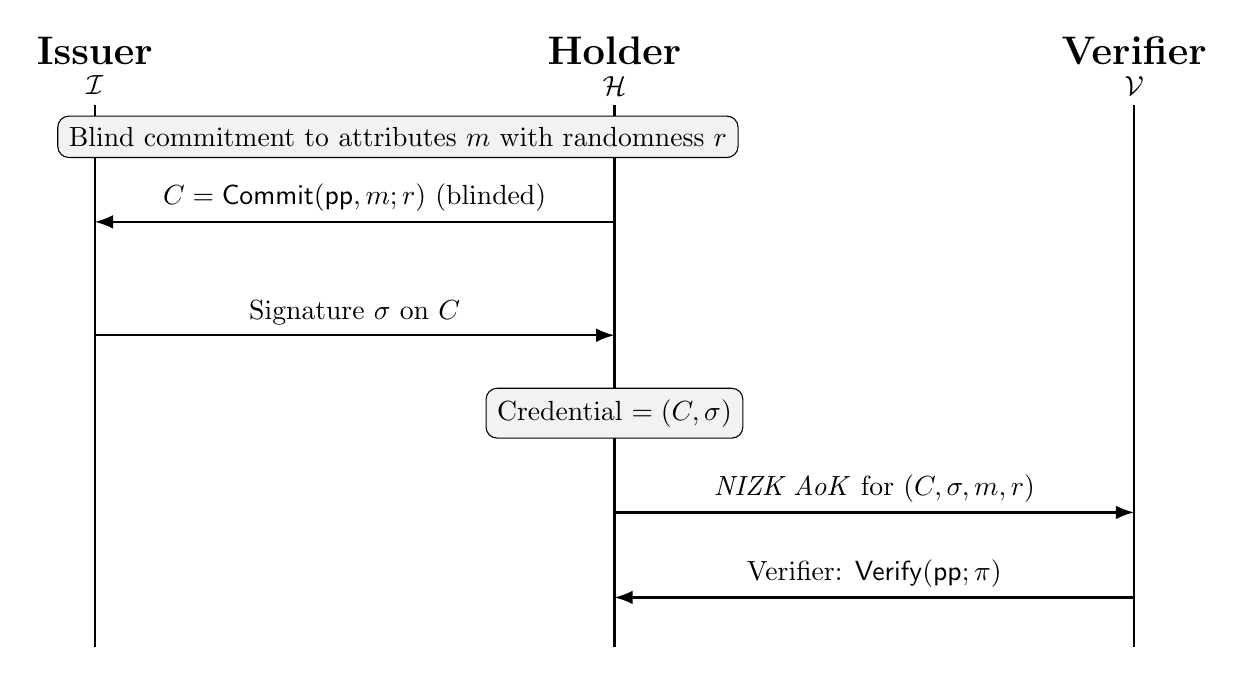
\begin{tikzpicture}[
    actor/.style={font=\bfseries, align=center},
    lifeline/.style={draw, thick},
    msg/.style={-Latex, thick},
    note/.style={draw, rounded corners, fill=gray!10, align=center, inner sep=4pt},
    tag/.style={font=\footnotesize\itshape},
    x=1.1cm, y=0.9cm
]
% --- Actors (Holder moved to the middle) ---
\node[actor] (I) at (0,0)  {\Large Issuer\\[-1pt]$\Issuer$};
\node[actor] (H) at (6,0)  {\Large Holder\\[-1pt]$\Holder$};
\node[actor] (V) at (12,0) {\Large Verifier\\[-1pt]$\Verifier$};

% --- Lifelines ---
\draw[lifeline] (I) -- ++(0,-8.2);
\draw[lifeline] (H) -- ++(0,-8.2);
\draw[lifeline] (V) -- ++(0,-8.2);

% --- Notes and messages ---
\node[note] at ($(H)+(-2.5,-1.0)$) {Blind commitment to attributes $m$ with randomness $r$};

% Commitment (Holder -> Issuer)
\draw[msg] ($(H)+(0,-2.2)$) -- node[above,sloped] {$C=\Commit(\PP,m;r)$ (blinded)} ($(I)+(0,-2.2)$);

% Signature (Issuer -> Holder)
\draw[msg] ($(I)+(0,-3.8)$) -- node[above,sloped] {Signature $\sigma$ on $C$} ($(H)+(0,-3.8)$);

\node[note] at ($(H)+(0,-4.9)$) {Credential $=(C,\sigma)$};

% Presentation (Holder -> Verifier)
\draw[msg] ($(H)+(0,-6.3)$) -- node[above,sloped] {\emph{NIZK AoK} for $(C, \sigma, m, r)$} ($(V)+(0,-6.3)$);

% Verification (Verifier -> Holder)
\draw[msg] ($(V)+(0,-7.5)$) -- node[above,sloped] {Verifier: $\Verify(\textsf{pp};\pi)$} ($(H)+(0,-7.5)$);

\end{tikzpicture}
\caption{Issuance and presentation flow. \emph{Default showing transmits only the proof~$\pi$; neither $r$ nor a deterministic tag is revealed, yielding unlinkability.}}
\label{fig:ac-flow}
\end{figure}

The public parameters for our construction are a trapdoored matrix \(\mathbf{A}\in R_q^{\,n\times m}\) (verification map) for an ISIS instance and a public matrix \(\mathbf{B}\in R_q^{\,n\times \ell}\) (hash domain).
The message and randomness are an ISIS preimage relation with a BBS-style \emph{rational hash}; its output \(\mathbf{t}\) serves as the commitment.
 For a message \(u\) and signing randomness
\(\chi\), the vSIS construction defines a rational function \(h_{u,\chi}\) and sets the target
\[
  \mathbf{t}\ \coloneqq\ h_{u,\chi}(\mathbf{B})\ \in R_q^{\,n}.
\]
A signature is precisely a short preimage \(\mathbf{s}\) such that
\[
  \boxed{\ \mathbf{A}\mathbf{s}\ \equiv\ \mathbf{t}\ \pmod q\ } \qquad\text{with}\quad \|\mathbf{s}\|\ \text{small}.
\]
This is the verification equation we will prove in zero knowledge later on.

Concrete choices of \(h_{u,\chi}\) translate the verification equations into low-degree
polynomial relations over \(R_q\)
% ; in our work, we use functions of the form
% $$h_{u,\chi}(\tilde{\mathbf{b}}_0,\tilde{\mathbf{b}}_1)
%   = \big((1,u^\top,x_0^\top)\cdot \tilde{\mathbf{b}}_0\big)\big/(\tilde{\mathbf{b}}_1-x_1)\text{,}$$
% with \(\chi=(x_0,x_1)\), which exactly yields an ISIS target \(\mathbf{t}\) when evaluated at the public
% parameter \(\mathbf{B}=(\mathbf{b}_0,\mathbf{b}_1)\).  
Previous work \cite{cryptoeprint:2025/356} formalizes this pattern through a
general signature skeleton \(\Sigma_{\mathrm{ISIS_f}}\) where verification checks \(\mathbf{A}\mathbf{s}=h_{u,\chi}(\mathbf{B})\pmod q\)
and \(\mathbf{s},\chi,u\) is short; our instantiation follows that template. 

\begin{comment}
\paragraph{Threat model (brief).}
We consider malicious holders (one-more unforgeability), malicious issuers (blindness), and verifiers (unlinkability). Security follows from SIS/ISIS hardness for signatures \cite{cryptoeprint:2025/356} and soundness/HVZK for SmallWood in ROM/FS \cite{cryptoeprint:2025/1085}.

\paragraph{Roadmap.}
Section~1 defines primitives (commitments, blind signatures, NIZK, SIS/ISIS, rational hash, vanishing polynomials). Section~2 covers algebraic preliminaries. Section~3 presents the vSIS-BBS scheme and the cleared identity. Section~4 details the Gaussian sampler. Section~5 reviews the SmallWood system (generic). Section~6 lists optimizations. Section~7 states parameter constraints and choices. Section~8 encodes vSIS-BBS in SmallWood (witness layout and constraints). Section~9 reports results.

\end{comment}
% 1. Preliminaries (definitions, SIS, commitments, NIZKs, blind sigs)
% \input{sections/01-algorithmic-defs}
% \section{Preliminaries II: Algebraic Setting and SIS/ISIS}
\label{sec:prelim-algebra}

\paragraph{Notation.}
Let $q\ge 2$ be an integer modulus and let $\varphi$ be a power of two.
We work in the cyclotomic ring $R \coloneqq \mathbb{Z}[X]/(X^\varphi+1)$ and its $q$-adic reduction
$R_q \coloneqq R/qR$. We use $\varphi$ exclusively for the ring degree and $N$ for the PCS/DECS domain size; when legacy formulas write $n$, read $n=\varphi$.
For vectors over $R$ we use boldface (e.g., $\mathbf{a}\in R^m$), and we write
$\|\cdot\|_2,\ \|\cdot\|_\infty$ for coefficient-wise norms on $R$ (extended component-wise to $R^m$).
Equalities “$\equiv \bmod q$” and Hadamard operations act coefficient-wise in the evaluation basis.
For a matrix $\mathbf{A}\in R_q^{k\times m}$ and target $\mathbf{t}\in R_q^k$, denote by
$\Lambda^\mathbf{t}_\perp(\mathbf{A}) \coloneqq \{\mathbf{e}\in R^m : \mathbf{A}\mathbf{e}\equiv \mathbf{t}\ (\bmod\ q)\}$ the corresponding coset of the lattice.


\paragraph{Convention (coefficient‑wise modeling).}
Via the NTT/evaluation basis we identify $R_q$ with $\F_q^N$; the Hadamard product $\Had$ and division $\Hdiv$ act component‑wise in that basis.
Equalities “$\equiv$ mod $q$” are understood coefficient‑wise unless stated otherwise.

\paragraph{Bounded alphabets and signed lifting.}
We fix an integer bound $B\ge 1$ and write
\[
[-B,B] := \{-B,-B{+}1,\ldots,0,\ldots,B\}\subset\mathbb{Z}.
\]
When encoding integers into $\mathbb{F}_q$, we use the \emph{signed lifting} $\langle i\rangle_q$ defined by
$\langle i\rangle_q = i \pmod q$ for $i\ge 0$ and $\langle i\rangle_q = q - ((-i)\pmod q)$ for $i<0$.

\subsection{SIS and ISIS (Ring Setting) and How We Instantiate Them}


\begin{definition}[SIS and ISIS over $R_q$]\label{def:sis-isis}
Fix integers $n,m\ge 1$ and a modulus $q\ge 2$, and work over $R_q$.
\begin{itemize}[leftmargin=1.25em]
  \item \textbf{SIS (homogeneous).} Given $\mathbf{A}\in R_q^{\,n\times m}$ and a bound $\beta>0$, find a nonzero $\mathbf{s}\in R^{m}$ such that $\mathbf{A}\mathbf{s}\equiv \mathbf{0}\pmod q$ and $\|\mathbf{s}\|\le\beta$ (for a prescribed norm, e.g., $\ell_\infty$ or $\ell_2$).
  \item \textbf{ISIS (inhomogeneous).} Given $(\mathbf{A},\mathbf{t})\in R_q^{\,n\times m}\times R_q^{\,n}$ and $\beta>0$, find $\mathbf{s}\in R^{m}$ with $\mathbf{A}\mathbf{s}\equiv \mathbf{t}\pmod q$ and $\|\mathbf{s}\|\le\beta$.
\end{itemize}
Hardness is measured against PPT adversaries; norms may be coefficient-wise $\ell_\infty$ or Euclidean $\ell_2$ as specified.
\end{definition}

\begin{definition}[Lattice trapdoor suite]\label{def:trapdoor}
Let $R_q=R/qR$. A lattice trapdoor suite consists of two PPT algorithms $(\TrapGen,\SampPre)$:
\begin{itemize}[leftmargin=1.25em]
  \item $(\mathbf{A},\mathsf{td}_\mathbf{A})\leftarrow \TrapGen(1^\lambda,1^n,1^m,q)$ outputs $\mathbf{A}\in R_q^{\,n\times m}$ statistically close to uniform together with a trapdoor $\mathsf{td}_\mathbf{A}$.
  \item $\mathbf{u}\leftarrow \SampPre(\mathsf{td}_\mathbf{A},\mathbf{v},s)$, on input $\mathbf{v}\in R_q^{\,n}$ and Gaussian parameter $s>0$, samples a short $\mathbf{u}\in R^{m}$ such that $\mathbf{A}\mathbf{u}\equiv \mathbf{v}\pmod q$.
\end{itemize}
For admissible parameters (as in GPV-type analyses), the output of $\SampPre$ is statistically close to the discrete Gaussian $D_{\Lambda^{\mathbf{v}}_{\perp}(\mathbf{A}),\,s}$. See, e.g., \cite{GPV08} for concrete admissibility conditions.
\end{definition}

\begin{remark}[Trapdoors]\label{rem:trapdoors-bridge}
In what follows we rely on $(\TrapGen,\SampPre)$ to sample short ISIS preimages and to argue statistical properties of signatures.
For a formal abstract statement see \Cref{def:trap-sampler}; our concrete ring/NTRU instantiation appears in \S\ref{sec:gaussian-preimage}.
\end{remark}

See also the abstract interface in Def.~\Cref{def:trap-sampler}.

\paragraph{From SIS/ISIS to our instantiation.}
Our signature core is an ISIS preimage relation with a BBS-style \emph{rational hash}; its output \(\mathbf{t}\) serves as the commitment image.
Public parameters include a trapdoored matrix \(\mathbf{A}\in R_q^{\,n\times m}\) (verification map) and a
public matrix \(\mathbf{B}\in R_q^{\,n\times \ell}\) (hash domain). For a message \(u\) and signing randomness
\(\chi\), the vSIS construction defines a rational function \(h_{u,\chi}\) and sets the target
\[
  \mathbf{t}\ \coloneqq\ h_{u,\chi}(\mathbf{B})\ \in R_q^{\,n}.
\]
A signature is precisely a short preimage \(\mathbf{s}\) such that
\[
  \boxed{\ \mathbf{A}\mathbf{s}\ \equiv\ \mathbf{t}\ \pmod q\ } \qquad\text{with}\quad \|\mathbf{s}\|\ \text{small}.
\]
This is the verification equation we will prove in zero knowledge later on.
Concrete choices of \(h_{u,\chi}\) translate the verification equations into low-degree
polynomial relations over \(R_q\); e.g., in the BBS-style line one has functions of the form
\(h_{u,\chi}(\tilde{\mathbf{b}}_0,\tilde{\mathbf{b}}_1)
  = \big((1,u^\top,x_0^\top)\cdot \tilde{\mathbf{b}}_0\big)\big/(\tilde{\mathbf{b}}_1-x_1)\),
with \(\chi=(x_0,x_1)\), which exactly yields an ISIS target \(\mathbf{t}\) when evaluated at the public
parameter \(\mathbf{B}=(\mathbf{b}_0,\mathbf{b}_1)\). The vSIS paper formalizes this pattern through a
general signature skeleton \(\Sigma_{\mathrm{ISIS_f}}\) where verification checks \(\mathbf{A}\mathbf{s}=h_{u,\chi}(\mathbf{B})\pmod q\)
and \(\mathbf{s}\) is short; our instantiation follows that template. 

\begin{definition}[Rational-hash commitment]
For message $u$ and signing randomness $\chi=(x_0,x_1)$, define
\[
  t\;\coloneqq\;h_{u,\chi}(B)\in R_q^n
\]
as the \emph{commitment} to $u$. The holder computes $t$ locally and reveals it only as required by the issuance/verification flow.\;\emph{Convention.} We call $h_{u,\chi}$ the \emph{rational hash} and $t$ its \emph{commitment image}.
\end{definition}

\paragraph{Sampling/representation conventions (as in \cite{cryptoeprint:2025/356}).}
Inside the proof, each component is restricted coefficient-wise to a bounded alphabet:
\[\nu \in [-B,B]^{kN},\qquad x_0 \in [-B,B]^{k_0N},\qquad x_1 \in [-B,B]^{N}.\]
(When $B{=}1$ this matches the balanced-ternary alphabet $\{-1,0,1\}$.)
We continue to compute $t=h_{u,\chi}(B)$ exactly in the NTT domain and resample $x_1$ until every coordinate of $b_1-x_1$ is invertible; the failure probability per coordinate is $(2B{+}1)/q$ and remains negligible.

\paragraph{Norm convention.}\label{par:norm-conv}
Unless explicitly stated otherwise, validity is checked via $\ell_\infty$ per coefficient (enforced by the chain gadget in \S\ref{sec:norm-gadget}). We choose the global Euclidean budget to conservatively imply the $\ell_2$ bound via
\[
\beta_2^2\ \ge\ T\,n\,B_\infty^2,
\]
where $T$ is the number of signature rows and $B_\infty$ follows from the chosen $(R,D,L)$ in the chain gadget.


\paragraph{Presentation unlinkability.} See the concrete \textsf{Show} in Section~\Cref{sec:encoding-vsis-smallwood}.

\subsection{Valid Preimage for Our ISIS Instantiation}
\label{subsec:valid-preimage-refined}
Let the public key fix \(\mathbf{A}\in R_q^{\,n\times m}\) and the public parameters fix \(\mathbf{B}\in R_q^{\,n\times \ell}\).
For a message \(u\) and randomness \(\chi\), define the vSIS–BBS hash target
\[
  \mathbf{t}\ \coloneqq\ h_{u,\chi}(\mathbf{B})\ \in R_q^{\,n},
\]
and the admissible witness set (for a chosen norm and bound \(\beta\))
\[
  \mathcal{W}_\beta(u,\chi)\ \coloneqq\ \Bigl\{\,\mathbf{s}\in R^{m}\ :\ \mathbf{A}\mathbf{s}\equiv \mathbf{t}\pmod q,\ \ \|\mathbf{s}\|\le \beta\,\Bigr\}.
\]
\begin{definition}[Valid preimage, ISIS–BBS]
A vector \(\mathbf{s}\in R^{m}\) is a \emph{valid preimage} for \((u,\chi)\) if
\(\mathbf{s}\in \mathcal{W}_\beta(u,\chi)\) i.e.,
\[
  \mathbf{A}\mathbf{s}\equiv h_{u,\chi}(\mathbf{B})\pmod q
  \quad\text{and}\quad
  \|\mathbf{s}\|_\infty\le \beta_\infty\ \ \text{(or }\|\mathbf{s}\|_2\le \beta_2\text{)}.
\]
\end{definition}
The bound \(\beta\) is chosen large enough for correctness under discrete-Gaussian preimage sampling
(\S\ref{subsec:gaussian}), yet small enough so that (i) the induced commitment/hash is computationally
binding, and (ii) our ZK constraints (the \(\ell_\infty\) gadget) remain efficient. In the vSIS
framework, \(\mathbf{t}=h_{u,\chi}(\mathbf{B})\) is produced by an algebraic, keyed rational function family,
and signatures are precisely short preimages for these images. 

\noindent In our BBS instantiation, the message subspace $\mathcal{M}_{X,\mathcal{H},B}$ simply enforces invertibility of each coordinate of $(b_1-x_1)$; we implement this by resampling $x_1$ until $(b_1-x_1)$ is slot-wise invertible (Algorithm~\ref{alg:compute-bbs-exact}, step~4).

\subsection{SmallWood Building Blocks (Quick Definitions)}
\label{subsec:smallwood-defs}
We rely on the following commitment/argument components:
\begin{itemize}[leftmargin=1.25em]
  \item \textbf{DECS} (Degree-Enforcing Commitment Scheme): a commitment layer that enforces low-degree structure of committed vectors/polynomials and supports proximity checks.
  \item \textbf{LVCS} (Linear Vector Commitment System): a vector commitment with linear operations and succinct openings; used to batch and route constraints.
  \item \textbf{PCS} (Polynomial Commitment Scheme): commit to a polynomial and prove evaluations/relations at points.
  \item \textbf{PIOP} (Polynomial IOP): an interactive oracle proof where the prover posts low-degree polynomials and the verifier queries them at random points; compiled via a PCS to a succinct (N)IZK.
\end{itemize}
SmallWood composes these layers (DECS\,$\rightarrow$\,LVCS\,$\rightarrow$\,PCS/PIOP) with hash-based commitments to obtain compact arguments and efficient norm gadgets for our use cases.

\subsection{Discrete Gaussian Preimage Sampling}
\label{subsec:gaussian}
\begin{definition}[Gaussian preimage sampler]\label{def:gaussian-sampler}
Given $(\mathbf{A},\mathsf{td}_\mathbf{A})$ and $\mathbf{t}\in R_q^{k}$, a Gaussian preimage sampler is a randomized algorithm
\[
  \mathsf{SamplePreimage}(\mathbf{A},\mathsf{td}_\mathbf{A},\mathbf{t};s)\ \longrightarrow\ \mathbf{e}\in \Lambda^{\mathbf{t}}_{\perp}(\mathbf{A})
\]
whose output distribution is statistically close to $D_{\Lambda^{\mathbf{t}}_{\perp}(\mathbf{A}),\,s}$ for a width $s$ above a scheme-dependent smoothing threshold. Such samplers (e.g., GPV and ring/NTRU refinements) underpin hash-and-sign signatures with overwhelming correctness and strong statistical properties.
\end{definition}

In practice we instantiate $\mathsf{SamplePreimage}$ with a ring–NTRU trapdoor and per-slot widths calibrated as in \S\ref{sec:gaussian-preimage}; our implementation is constant-time in the coefficient domain.

\lena{
\subsection{Anonymous Credentials}
Anonymous credentials allow users to prove possession of valid credentials without revealing their identity or enabling linking across presentations. A foundational primitive for such systems is a Signature with Efficient Protocols~(SEP)~\cite{SCN:CamLys02}. A SEP is a signature scheme that supports efficient evaluation and ZKPs of possession of a valid signature in a two-party setting. SEPs allow the creation of a digital credential, where a user can prove they possess a valid credential without revealing which specific credential or any identifying information. 

A basic anonymous credential supports only a single presentation: after one use, subsequent presentations become linkable to the first since the same proof would be shown again. To achieve \emph{multi-show credentials} with unlinkable presentations, the construction must incorporate a mechanism to ensure each presentation appears independent while preventing unlimited reuse.

Recent IETF standardization efforts address multi-show credentials through Anonymous Rate-Limited Credentials~(ARC)~\cite{draft-yun-privacypass-crypto-arc-00}. ARC enables a single credential issuance to support multiple unlinkable presentations, up to a configurable limit. Each presentation uses a fresh nonce and randomization to ensure unlinkability, while the server enforces rate limits by tracking presentation-specific tags. 

Since SPRUCE provides a signature scheme with efficient proof protocols, we aim to construct a post-quantum SEP and subsequently a post-quantum variant of ARC.

@Carsten: not sure about the proofs. I added more context on ARC in~\Cref{sec:anonymous-credentials}
}
\section{Preliminaries - a'la Carsten}
\label{sec:prelims}
\paragraph{Notation.}
We let $\negl(n)$ denote any positive function that is negligible in $n$, i.e. upper-bounded by $1/|p(n)|$ for any polynomial $p$ and large enough $n$. Let $\lambda$ denote the security parameter and we write PPT to denote probabilistic algorithms whose runtime is polynomial in $\lambda$. For $a,b\in \mathbb{Z},a<b$ write $[a,b]$ to denote the set $[a,a+1,\dots,b-1,b]$ and use $[b]$ as a short-hand for $[1,b]$.


\subsection{Commitment Schemes}\label{subsec:commit}

\begin{definition}[Non-interactive commitment]\label{def:commit}
A \emph{commitment scheme} consists of the following polynomial-time algorithms:
\begin{itemize}
    \item $\Setup(\SecParam)\rightarrow \PP:$ Takes the security parameter as input and outputs a commitment public key $\PP$. $\PP$ also describes the message space $\ComMsg$, randomness space $\ComRand$ and commitment space $\ComSpace$.
    \item $\Commit(\PP,\mu,r) \rightarrow c:$ Takes a commitment public key $\PP$, a message $\mu\in \ComMsg$ and randomness $r\in \ComRand$ as input and outputs a commitment $c\in\ComSpace$.
\end{itemize}
\end{definition}

We say that a commitment scheme is correct if for any honestly generated $\PP$, the algorithm $\Commit$ is deterministic and always terminates except with negligible probability. In addition, we require that it is binding and hiding:
\begin{definition}[Binding]\label{def:binding}
    A commitment scheme $(\Setup,\Commit)$ is \emph{binding} if there exists a negligible function $\negl$, such that for any PPT algorithm $\adversary$ we have that  \[
        \Pr \left[ \begin{matrix} c_1 = c_2, \\ c_1\neq \bot, \, \mu_1\neq \mu_2 \end{matrix} \, \middle | \, \begin{matrix}
            \PP \gets \Setup(\SecParam), \\
            (\mu_1,\mu_2,r_1,r_2) \gets \adversary(\PP),\\
            c_1 \gets \Commit(\PP, \mu_1, r_1),\\
            c_2 \gets \Commit(\PP, \mu_2, r_2)
        \end{matrix} \right] \leq \negl(\lambda) \, .    
    \] 
\end{definition}

\begin{definition}[Hiding]\label{def:hiding}
    A commitment scheme $(\Setup,\Commit)$ is \emph{hiding} if there exists a negligible function $\negl$, such that for any PPT algorithm $\adversary$ we have that  \[
       \left| \Pr \left[  b = \adversary(c, \state)  \, \middle | \, \begin{matrix}
            \PP \gets \Setup(\SecParam), \\
            (\mu_0,\mu_1,\state)\gets \adversary(\PP), \\
            b\getsunif \{0,1\},\, r\getsunif \ComRand, \\
            c \gets \Commit(\PP,\mu_b,r)  )
        \end{matrix} \right] -\frac{1}{2} \right|     
    \] 
    is bounded by $\negl(\lambda)$.
\end{definition}



\subsection{Blind Signatures} \label{subsec:blind}


We provide the correctness and security definitions of Blind signatures~\cite{C:Chaum82}. 

\begin{definition}[Blind Signature]\label{def:blind}
A round-optimal \emph{Blind signature} scheme consists of the following five PPT algorithms:

\begin{itemize}
    \item $\KeyGen(\SecParam)\rightarrow (\sk,\pk):$ Takes the security parameter as input and outputs a secret key $\sk$ and a public key $\pk$.
    \item $\Sign_1(\pk,\mu) \rightarrow (\rho_1,S_\User):$ This is the first part of a signing protocol between a user $\User$ and a signer $\Signer$, where $\User$ uses a public key and a message $\mu \in \{0,1\}^\ast$, to compute a state $S_\User$ and a first message $\rho_1$, which they send to $\Signer$.
    \item $\Sign_2(\sk, \rho_1) \rightarrow \rho_2 :$ The second part of the interaction, where $\Signer$ uses their signing key $\sk$ and a first message $\rho_1$ and outputs a second message $\rho_2$, which they send to $\User$.
    \item $\Sign_3(\rho_2, S_\User) \rightarrow \sig:$ The last part of the interaction, where $\User$ uses $\rho_2$ and $S_\User$ to derive a signature $\sig$ or $\bot$ if the signing protocol failed.
    \item $\Verify(\pk,\mu,\sig) \rightarrow \{0,1\}$: A verification algorithm that takes as input a public key $\pk$, a message $\mu$ and a signature $\sig$ and outputs a bit to indicate whether the signature is deemed valid (1) or invalid (0).
\end{itemize}

All the algorithms take the security parameter $\lambda$ as input (sometimes implicitly).
\end{definition}

We require Blind signatures to satisfy three properties: correctness, which says that honestly generated signatures should verify with probability close to 1, blindness, which says that the signer cannot link signatures to the interaction with which they were created, and existential unforgeability, which says that if a user is allowed to execute the signing protocol $Q$ times with chosen messages it cannot obtain valid signatures for any other messages.

\begin{definition}[Correctness] \label{def:bs-correctness}
    A Blind signature $(\KeyGen,(\Sign_i)_{i\in [3]},\Verify)$ is \emph{correct} if there exists a negligible function $\negl$, such that for any message $\mu$ we have \[
        \Pr \left[ \Verify(\pk,\mu,\sig) = 1 \, \middle | \, \begin{matrix}
            (\sk,\pk) \gets \KeyGen(\SecParam), \\
            (\rho_1, S_\User) \gets \Sign_1(\pk, \mu), \\
            \rho_2 \gets \Sign_2(\sk, \rho_1), \\
            \sig \gets \Sign_3(\rho_2, S_\User)
        \end{matrix} \right]    
    \] 
    is  $1$  except with probability $\negl(\lambda)$.
\end{definition}


\begin{definition}[Blindness] \label{def:bs-blindness}
    A Blind signature $(\KeyGen,(\Sign_i)_{i\in [3]},\Verify)$ has \emph{blindness} if for every polynomial-time three-part stateful adversary $\adversary = (\adversary_1, \adversary_2, \adversary_3)$ there exists a negligible function $\negl$ such that for any two messages $\mu_0, \mu_1$ we have \[
        \left| \Pr\left[ \adversary_3(\sig^0,\sig^1) = b \, \middle| \,
        \begin{matrix} 
            \pk \gets \adversary_1(\SecParam), b \getsunif \{0,1\}, \\
            (\rho_1^0, S_\User^0) \gets \Sign_1(\pk,\mu_0), \\ (\rho_1^1, S_\User^1) \gets \Sign_1(\pk,\mu_1), \\
            \rho_2^b,\rho_2^{1-b} \gets \adversary_{2}( \rho_1^b, \rho_1^{1-b} ), \\
            \sig^0 \gets \Sign_3(\rho_2^0, S_\User^0), \\
            \sig^1 \gets \Sign_3(\rho_2^1, S_\User^1), \\
            \text{If } \bot \in \{ \sig^0,\sig^1\} \\  \text{ then } (\sig^0,\sig^{1}) \gets (\bot,\bot) \\
        \end{matrix} \right] - \frac{1}{2} \right|
    \]
    is bounded by $\negl(\lambda)$.
\end{definition} 



\begin{definition}[One-more unforgeability] \label{def:bs-unforgeability}
    A Blind signature $(\KeyGen,\allowbreak (\Sign_i)_{i\in [3]},\allowbreak \Verify)$ is \emph{one-more unforgeable} if for every polynomial-time adversary $\adversary$ making at most $Q$ queries ($Q$ is a function of $\lambda$, bounded by a polynomial) to the signing oracle $\Sign_2$ there exists a negligible function $\negl$ such that \[
    \Pr\left[ \begin{matrix} \forall 1 \leq i < j \leq Q+1 : \\ \left( \mu_i \neq \mu_j \right) , \\
        \forall 1 \leq i \leq Q+1 : \\ \left( \Verify(\pk, \mu_i, \sig_i) = 1 \right)\\
    \end{matrix}  \, \middle| \, \begin{matrix}
        (\sk,\pk) \gets \KeyGen(1^\lambda), \\
        \{(\mu_i,\sig_i)\}_{i \in [Q+1]} \gets  \\
        \,\, \adversary^{\Sign_2(\sk,\cdot))}(\pk) \\ 
    \end{matrix} \right] \leq \negl(\lambda) \, .
    \]
\end{definition} 



\subsection{Non-Interactive Zero-Knowledge Arguments}\label{subsec:nizk}
We now describe the model of Non-Interactive Zero-Knowledge Arguments (NIZKs) that we use in this work.

\paragraph{Computational model.}
We model computation by applying a circuit  $C$ to an input $\vw\in \Z_q^{\ell}$. $C$ has $\ell$ input wires and a single output wire. We say that the input $\vw$, or witness, is valid if $C(\vw)=0$ and invalid otherwise.


$C$ consists of wires and gates, where each gate has at least one input wire and exactly one output wire. The input wires of each gate are either the input wires of $C$, or output wires of other gates. The output of a gate may be input to multiple other gates, and the wires and gates form an acyclic directed graph. There are $3$ types of gates in a circuit:
\begin{description}
\item[Linear gates] apply public linear functions $\mathtt{lin}(\valpha,\beta,\vx)=\langle \valpha,\vx\rangle +\beta$ on the input wires $\vx\in \Z_q^h$. $\valpha \in \Z_q^h, \beta \in \Z_q$ are public inputs to the gate, while the output is a single element in $\Z_q$. Note that $h$ may be arbitrarily large.
\item[Multiplication gates]  take as input a vector $\vx \in \Z_q^h$, compute the product of all input wires $\mathtt{mul}(\vx)=\prod_{i\in[h]} x_i $ and output the product as an element in $\Z_q$. $h$ can be larger than 2.
\item[Assert gates] take as input a wire value $x\in \Z_q$ and output $\top$ if $x=0$ and $\bot$ otherwise. Note that the output wire of an assert gate may therefore never be input to another gate.
\end{description}

We define the evaluation of $C$ on input $\vw$ as follows:  $\vw$ is initially assigned to the input wires of the circuit, and then consecutively all gates whose input wires are fully assigned are evaluated and the output of the gate function is assigned to the output wire(s).
This process is repeated until a) the single output wire of the circuit has a value assigned to it; and b) all \emph{assert gates} have been evaluated. If all assert gates have output $\top$ then $C(\vw)$ is equivalent to the value assigned to the output wire of $C$, otherwise $C(\vw)=\bot$.

\paragraph{NIZKs.}
We now define NIZK proof systems in the random oracle (RO) model. 
\begin{definition}\label{def:nizk}
A \emph{NIZK proof system} $\Pi$  is a tuple $\Pi = ( \Prove, \Verify)$ of PPT algorithms that have access to the random oracle $\RO$:
\begin{itemize}
    \item $\Prove^{\RO}(C,\vw) \rightarrow \pi$: Takes a circuit $C$ and a witness $\vw$  and outputs a proof $\pi$.
    \item $\Verify^{\RO}(C,\pi) \rightarrow \{0,1\}$: Takes a circuit $C $, and a proof $\pi$, and outputs a bit to indicate whether the proof is deemed valid ($1$) or invalid ($0$).
\end{itemize}
\end{definition}
In the following, we drop the superscript $\RO$ from $\Prove,\Verify$ to simplify notation.

\begin{definition}[Correctness]
    \label{def:nizk-correctness}
    A NIZK proof system $(\Prove, \Verify)$ in the RO model has \emph{correctness error} $\correrr$
    if for any $C$ and for all $\vw\in \F_q^\ell$ such that $C(\vw)=0$,
    \begin{equation*}
        \Pr\left[
        \Verify( C,\pi) = 1
        \middle |
           \pi\gets \Prove(C,\vw)
         \right]
        \geq 1 - \correrr(\SecParam)
    \end{equation*}
    $( \Prove, \Verify)$ is \emph{correct} if $\correrr = \negl$.
\end{definition}


\begin{definition}[Non-interactive Zero-Knowledge]\label{def:nizk-zk}
    A simulator $\Sim$ for a NIZK proof system $\Pi = ( \Prove, \Verify)$  is a  PPT algorithm  with implicit input $\SecParam$.
    $\Sim$ on input $C$ outputs $\pi$.
    Let $\adversary$ be a stateful algorithm and let
    \begin{equation*}
        \begin{aligned}
            \Real_{\adversary}(\SecParam) &= \Pr%\left[
            \begin{bmatrix}
               b=1 \, | \, b \gets \adversary^{\RO, \mathcal{O}_{\Prove}}(\SecParam)
                     \end{bmatrix} \\
/            \Ideal_{\adversary}(\SecParam) &= \Pr%\left[
            \begin{bmatrix}
               b=1 \, | \, b \gets \adversary^{\RO, \mathcal{O}_{\Sim}}(\SecParam)
            \end{bmatrix}
            % \right]
        \end{aligned}
    \end{equation*}
    The adversary has black-box access to the random oracle $\RO$ and to an oracle $\mathcal{O}_{\Prove}$ or $\mathcal{O}_{\Sim}$. These oracles take $C,\vw$ as input, check if $C(\vw)=0$ and then do the following: 
    \begin{itemize}
        \item $\mathcal{O}_{\Prove}(C,\vw)$ computes $\pi \gets \Prove^{\RO}(C,\vw)$ and outputs $\pi$.
         \item $\mathcal{O}_{\Sim}(C,\vw)$ computes $\pi\gets \Sim^{\RO}(C)$.
    \end{itemize}
    The simulator $\Sim$ is allowed to \emph{program} the random oracle $\RO$ on any fresh input to $\RO$,
       i.e.\ if $\RO(m)$ has not been queried by any party before, then $\adversary$ resp.\ $\Sim$ is free to choose $\RO(m)$, otherwise, programming fails. 
       
    We define the advantage of $\adversary$ by $ \left|\Real_{\adversary}(\SecParam) - \Ideal_{\adversary}(\SecParam)\right|$.
    We call $\Sim$ a \emph{Non-interactive Zero-Knowledge Black-box} simulator for $\Pi$
    if for any PPT $\adversary$ the advantage is negligible.
\end{definition}
Knowledge soundness for \emph{black-box} extraction in the  RO model for NIZKs is defined as follows:


\begin{definition}
    \label{def:nizk-knowledge}
    Let $\Pi$ be a non-interactive proof system and $\KExt$ be a  PPT algorithm. 
    Define the knowledge soundness experiment as follows:
    \begin{enumerate}
    \item The experiment obtains $C$  as input.
    \item Run $\adversary^{\RO}(\SecParam,C)$ until it outputs $\pi$. Let $Q$ be all RO queries made by $\adversary$.
    \item Return $0$ if $\Verify(C,\pi)=0$.
        \item Return $1$ if   $C(\KExt(C, \pi, Q))\neq 0$, else return $0$.
    \end{enumerate}
    The advantage of $\adversary$ is defined as the probability that the experiment returns $1$.
    If there exist $\KExt$ such that for every PPT $\adversary$ the advantage is negligible,     then we call $\Pi$ knowledge sound.

\end{definition}




\subsection{Lattice Primitives}

\paragraph{Lattice preliminaries and evaluation basis.}
Let $q\ge 2$ be an integer modulus and let $\varphi$ be a power of two. We work in the cyclotomic ring
$R \coloneqq \Z[X]/(X^\varphi+1)$ and its $q$-adic reduction $R_q \coloneqq R/qR$. For vectors over $R$ we use
boldface (e.g.\ $\mathbf{a}\in R^m$), and we write $\|\cdot\|_2,\ \|\cdot\|_\infty$ for coefficient-wise norms on $R$
(extended component-wise to $R^m$). Via the NTT/evaluation basis, Hadamard product $\odot$ and Hadamard
division $\oslash$ act coordinate-wise; division is understood only when all denominator coordinates are nonzero.

\medskip
We work with a NTT-friendly prime $q$ such that :
\[
\operatorname{ord}_{\,2\varphi}(q)=1 \quad\Longleftrightarrow\quad q\equiv 1 \pmod{2\varphi}.
\]

We thus can identify $R_q \cong \F_q^{N}$ (with $N=\varphi$) since the cyclotomic polynomial $X^\varphi+1$ splits completely over $\F_q$.

% Equalities “$\equiv$ mod $q$” are understood coefficient‑wise unless stated otherwise.

\begin{definition}[SIS and ISIS over $R_q$]\label{def:sis-isis}
Fix integers $n,m,\varphi\ge 1$ where $\varphi$ is a power of $2$ and let  $q\ge 2$ be a modulus. Define $R_q$ as above.
\begin{itemize}[leftmargin=1.25em]
  \item \textbf{The homogeneous SIS  problem.} Given $\mathbf{A}\in R_q^{\,n\times m}$ and a bound $\beta>0$, find a non-zero $\mathbf{s}\in R^{m}$ such that $\mathbf{A}\mathbf{s}\equiv \mathbf{0}\pmod q$ and $\|\mathbf{s}\|\le\beta$ (for a prescribed norm, e.g., $\ell_\infty$ or $\ell_2$).
  \item \textbf{The inhomogeneous SIS (ISIS) problem.} Given $(\mathbf{A},\mathbf{t})\in R_q^{\,n\times m}\times R_q^{\,n}$ and $\beta>0$, find $\mathbf{s}\in R^{m}$ with $\mathbf{A}\mathbf{s}\equiv \mathbf{t}\pmod q$ and $\|\mathbf{s}\|\le\beta$.
\end{itemize}
We say that an attacker $\adversary$ solves the SIS problem if $\adversary$, on input $\mathbf{A},\beta$ as well as all parameters of the SIS instance, outputs a valid solution $\mathbf{s}$. A similar definition can be made for the ISIS problem. On a formal level, we will assume that for the SIS/ISIS instances that we use, no PPT algorithm $\adversary$ solves them with non-negligible advantage. Concretely, we will later choose $q,n,m,\varphi$ such that attacks require a runtime of at least $2^{\lambda}$.
\end{definition}

\subsubsection{Trapdoors}

Let $\mathbf{c}\in \mathbb{R}^m$ and $s>0$, then the Gaussian function on $\mathbb{R}^m$ with center $\mathbf{c}$ and parameter $s$ is defined as 
\[
\forall \mathbf{x}\in \mathbb{R}^m:~ \rho_{s,\mathbf{c}}(\mathbf{x}):=\exp{-\pi \|\mathbf{x}-\mathbf{c}\|^2/s^2}\text{.}
\]
\begin{definition}[Discrete Gaussian Distribution]
For any $\mathbf{c}\in \mathbb{R}^m$, real $s>0$ and $m$-dimensional lattice $\Lambda$, the  \emph{discrete Gaussian distribution} over $\Lambda$ is defined as
\[
\forall \mathbf{x}\in \Lambda:~ D_{\Lambda,s,\mathbf{c}}:=\dfrac{\rho_{s,\mathbf{c}}(\mathbf{x})}{\rho_{s,\mathbf{c}}(\Lambda)}
\]
\end{definition}
If $\mathbf{c}=\mathbf{0}$, i.e. the distribution is centered, then we drop $\mathbf{c}$ from the definition.


For a matrix $\mathbf{A}\in R_q^{n\times m}$ and target $\mathbf{t}\in R_q^{n}$, denote by
$\Lambda^\mathbf{t}_\perp(\mathbf{A}) \coloneqq \{\mathbf{e}\in R^m : \mathbf{A}\mathbf{e}\equiv \mathbf{t}\ (\bmod\ q)\}$ the corresponding coset of the lattice.


\begin{definition}[Lattice trapdoor suite]\label{def:trapdoor}
Let $R_q=R/qR$. A lattice trapdoor suite consists of two PPT algorithms $(\TrapGen,\SampPre)$:
\begin{itemize}[leftmargin=1.25em]
  \item $(\mathbf{A},\mathsf{td}_\mathbf{A})\leftarrow \TrapGen(1^\lambda,1^n,1^m,q)$ outputs $\mathbf{A}\in R_q^{\,n\times m}$  together with a trapdoor $\mathsf{td}_\mathbf{A}$.
  \item $\mathbf{u}\leftarrow \SampPre(\mathsf{td}_\mathbf{A},\mathbf{v},s)$, on input $\mathbf{v}\in R_q^{\,n}$ and 
  parameter $s>0$, samples a vector  $\mathbf{e}\in \Lambda^{\mathbf{t}}_{\perp}(\mathbf{A})$.
\end{itemize}

\end{definition}

We now define security for  trapdoor sampler:
\begin{definition}[Secure Trapdoor sampler]
    Let $(\TrapGen,\SampPre)$ be a lattice trapdoor suite. 
Let $\adversary$ be any algorithm and let
    \begin{equation*}
        \begin{aligned}
            \Real_{\adversary}(\SecParam) &= \Pr%\left[
            \begin{bmatrix}
               b=1 \, | \, b \gets \adversary^{\mathcal{O}_{\Real,G},\mathcal{O}_{\Real,S}}(\SecParam)
                     \end{bmatrix} \\
            \Ideal_{\adversary}(\SecParam) &= \Pr%\left[
            \begin{bmatrix}
               b=1 \, | \, b \gets \adversary^{\mathcal{O}_{\Ideal,G},\mathcal{O}_{\Ideal,S}}(\SecParam)
            \end{bmatrix}
            % \right]
        \end{aligned}
    \end{equation*}
    The adversary has black-box access to two pairs of oracles. These oracles do the following
    \begin{itemize}
        \item $\mathcal{O}_{\Real,G}()$ upon first call computes $(\mathbf{A},\mathsf{td}_\mathbf{A})\gets \TrapGen()$, stores them and outputs $\mathbf{A}$. It ignores all further calls.
        \item $\mathcal{O}_{\Real,S}()$ samples $\mathbf{v}\gets R_q^n$ uniformly at random, computes $\mathbf{s}\gets \SampPre(\mathsf{td}_\mathbf{A},\mathbf{v},s)$ and outputs $(\mathbf{s},\mathbf{v})$.
                \item $\mathcal{O}_{\Ideal,G}()$ upon first call samples $\mathbf{A}\gets R_q^{n\times m}$ uniformly at random, stores $\mathbf{A}$ and outputs it. It ignores all further calls.
        \item $\mathcal{O}_{\Ideal,S}()$ samples $\mathbf{e}\gets D_{\Lambda_\bot^\mathbf{t}(\mathbf{A}),s}$, compute $\mathbf{v}= \mathbf{A}\mathbf{e}$ and outputs $(\mathbf{s},\mathbf{v})$.
    \end{itemize}
       
    We define the advantage of $\adversary$ by $ \left|\Real_{\adversary}(\SecParam) - \Ideal_{\adversary}(\SecParam)\right|$.
    We call the trapdoor suite \emph{secure} if for any potentially computationally unbounded $\adversary$, the advantage is negligible.

\end{definition}


\subsubsection{Rational Hashes}

\begin{definition}[Rational hash family $H$]\label{def:rational-hash}
Fix public $B=(B_0,b_1)\in R_q^{n\times \ell}$, message $u$, and randomness $\chi=(x_0,x_1)$ in prescribed ranges.
Define $h_{u,\chi}: R_q^{n\times \ell}\to R_q^n$ by
\[
  h_{u,\chi}(B)\;=\; B_0\cdot(1;u;x_0)\ \oslash\ \bigl(b_1-\mathbf{1}_n\cdot x_1\bigr),
\]
% where $\oslash$ denotes \emph{Hadamard} (slot-wise) division in the evaluation basis.
The denominator is required to
be nonzero in \emph{every} slot (i.e., coordinate-wise invertible in $R_q$). We call $h_{u,\chi}$ the \emph{rational hash}
and $t=h_{u,\chi}(B)$ the \emph{commitment image} of $(u,\chi)$.
\end{definition}



\paragraph{Security assumptions for rational hashes.}
Our $H=\{h_{u,\chi}\}$ is analyzed in the framework given by A.Dubois \emph{et.al} \cite{cryptoeprint:2025/356} as follows.

\begin{itemize}
  \item \textbf{Natural predicate $P_{\gamma,\varepsilon}$.} We restrict function sets by the predicate
  $P_{\gamma,\varepsilon}$: (i) the family is $\varepsilon$-\emph{strongly linearly independent} (SLI) and (ii) every denominator polynomial has coefficients bounded by $\gamma$. This prevents degenerate
  choices (e.g.\ adaptively zeroing denominators) and rules out linear-dependency pitfalls. \cite[Defs~6-7]{cryptoeprint:2025/356}
  % \cite[Def6-7]

  \item \textbf{Hinted vSIS hardness.} For function families augmented with $P_{\gamma,\varepsilon}$, the signature’s
  EUF security reduces to \emph{strong} hinted-vSIS (s-Hint-vSIS): given short preimages of $Q$ hints
  $\{h_{u_i,\chi_i}(B)\}$, producing a short preimage for a \emph{fresh} target $h_{u^\star,\chi^\star}(B)$ is hard. \cite[§3.1]{cryptoeprint:2025/356}
  % cite par.3.1]

  \item \textbf{Equivalence to GenISIS\textsubscript{$f$}.} Our concrete family $h_{u,\chi}(B)$ instantiates $f(\cdot)$ in the
  generalized ISIS\textsubscript{$f$} assumption, and s-EUF-RMA of the vSIS scheme is \emph{equivalent} to GenISIS\textsubscript{$f$}
  (and conversely to s-$\,\$\,$Hint-vSIS under the same parameters). This pins the security definition to a standard
  preimage-resistance style assumption with oracle access. \cite[Thm~7-8]{cryptoeprint:2025/356}
  % Thm7-8]

  \item \textbf{SLI in practice.} When $R_q$ \emph{splits} into a product of fields, ordinary
  linear independence implies SLI with explicit $\varepsilon$. This corresponds to the setting induced by
  the condition : $q\equiv 1\bmod 2\varphi$. 
  % Thm1 footnote on splitting

  \item \textbf{Robustness note.} The work from A.Dubois \emph{et.al} also analyzes linear-combination attacks and shows why the “natural’’
  predicate (denominator bound + SLI) is the right guardrail for rational families (e.g., BB/BBS-type forms),
  ensuring that easy linear relations in $\operatorname{im}(h_{u,\chi})$ do not yield short forgeries. 
  
  
\end{itemize}

% \todo[inline]{does this have a security definition?}

\paragraph{Signed Lifting} When encoding integers into $\mathbb{F}_q$,  the \emph{signed lifting} $\langle i\rangle_q$ is defined by
$\langle i\rangle_q = i \pmod q$ for $i\ge 0$ and $\langle i\rangle_q = q - ((-i)\pmod q)$ for $i<0$.


\begin{definition}[Vanishing polynomial for set membership]\label{def:vanish}
For a bound $B\in\mathbb{Z}_{>0}$, define
\[
  P_B(X)\;=\;\prod_{i=-B}^{B}\bigl(X-\langle i\rangle_q\bigr)\ \in \mathbb{Z}_q[X].
\]
For any $x\in\mathbb{Z}_q$, the predicate $x\in[-B,B]$ (w.r.t.\ signed lifting) is equivalent to 
$P_B(x)\equiv 0\pmod q$.
\end{definition}

When instantiating the rational hash, each component is restricted coefficient-wise to a bounded alphabet:
\[u \in [-B,B]^{kN},\qquad x_0 \in [-B,B]^{k_0N},\qquad x_1 \in [-B,B]^{N}.\]
A verifier can therefore validate that $t$ is well-formed by verifying a ZK argument of knowledge of a preimage $u,x_0,x_1$ which fulfill the aforementioned bounds, where the computed circuit is given by Definition \ref{def:vanish}.

\begin{comment}
Inside the proof, each component is restricted coefficient-wise to a bounded alphabet:
\[\nu \in [-B,B]^{kN},\qquad x_0 \in [-B,B]^{k_0N},\qquad x_1 \in [-B,B]^{N}.\]
(When $B{=}1$ this matches the balanced-ternary alphabet $\{-1,0,1\}$.)
We continue to compute $t=h_{u,\chi}(B)$ exactly in the NTT domain and resample $x_1$ until every coordinate of $b_1-x_1$ is invertible; the failure probability per coordinate is $(2B{+}1)/q$ and remains negligible.
\end{comment}






% % 2. vSIS--BBS blind signature scheme (with PKC adaptations)
% \input{sections/03-vsis-bbs}

% 3. Gaussian sampler
\section{Gaussian Preimage Sampler for vSIS–BBS (Antrag–Hybrid over NTRU)}
\label{sec:gaussian-preimage}

The first main primitive of our scheme is the Gaussian pre-image sampler used by our signature construction.
At a high level, given a public linear map \(\mathbf{A}\in R_q^{\,n\times m}\) and a target \(\mathbf{t}\in R_q^{\,n}\) produced by the vSIS–BBS hash, we sample a short vector \(\mathbf{s}\in R^{m}\) such that
\[
  \mathbf{A}\mathbf{s}\ \equiv\ \mathbf{t}\pmod q,
\quad\text{i.e.,}\quad
  \mathbf{s}\ \in\ \Lambda_{\perp}^{\mathbf{t}}(\mathbf{A}) \coloneqq \{\,\mathbf{x}\in R^{m}:\mathbf{A}\mathbf{x}\equiv\mathbf{t}\ (\bmod q)\,\}.
\]
Our concrete sampler is a ring–NTRU instantiation of Prest’s \emph{hybrid} two-plane Gaussian sampler with the \emph{Antrag} trapdoor-generation method, which attains high trapdoor quality while keeping key generation simple and fast (cf.\ \cite{cryptoeprint:2025/356}). The parameters that we need to control for said sampler are per-coefficient standard deviation of the distributions and the outputed norm of the pre-image. 


\subsection{NTRU trapdoor form and quality}
\label{subsec:trapdoor-form}

We work with the standard rank-2 NTRU module over the cyclotomic ring \(R=\mathbb{Z}[X]/(X^n+1)\) and its reduction \(R_q\).  An NTRU public key is \(h=g f^{-1}\bmod q\) for secret \(f,g\in R\), and the corresponding module is
\[
  \mathsf{L}_{\mathsf{NTRU}}(h)\ =\ \{(u,v)\in R^2 : u h - v \equiv 0 \ (\bmod q)\}.
\]
A \emph{trapdoor basis} of \(\mathsf{L}_{\mathsf{NTRU}}(h)\) is
\[
  B_{f,g}\ \coloneqq\
  \begin{pmatrix}
    f & F\\[2pt]
    g & G
  \end{pmatrix},
  \qquad\text{with}\qquad fG - gF \ =\ q,
\]
whose first column \((f,g)\) and second column \((F,G)\) are short and satisfy \(g/f \equiv G/F \equiv h \pmod q\).  The trapdoor \((f,g;F,G)\) is \emph{good} when its quality \(\alpha\) is close to \(1\), where
\[
  \alpha^{2}\ =\ \max_{1\le i\le d}\, 
  \max\!\left\{\
    \frac{|{\varphi_i(f)}|^2+|{\varphi_i(g)}|^2}{q},
    \frac{q}{|{\varphi_i(f)}|^2+|{\varphi_i(g)}|^2}
  \right\},
\]
i.e., each slot energy \(S_i\coloneqq |{\varphi_i(f)}|^2+|{\varphi_i(g)}|^2\) lies in the window
\[
  \frac{q}{\alpha^2}\ \le\ S_i\ \le\ \alpha^2 q
  \qquad\text{for all embeddings } \varphi_i.
\]
Equivalently, \((|\varphi_i(f)|,|\varphi_i(g)|)\) lies in the \emph{annulus arc}
\(A^+(\sqrt{q}/\alpha,\ \alpha\sqrt{q})\subset\mathbb{R}_{\ge0}^2\).  With this metric, the hybrid sampler’s Gaussian width scales essentially like \(\alpha\sqrt{q}\): smaller \(\alpha\) means tighter signatures and higher security for a fixed \(q,n\).

% ===================== Sampler (definition + tuning) FIRST =====================
\subsection{Sampler definition and parameter tuning}
\label{subsec:tuning}

\paragraph{Definition (hybrid two‑plane).}
Given $(\mathbf{A},\mathsf{td})$ and a target $\mathbf{t}$, the signer runs a ring‑based two‑plane sampler in the evaluation domain:
\[
  \mathsf{SamplePreimage}(\mathbf{A},\mathsf{td},\mathbf{t}; \{\sigma_k[i]\})\ \longrightarrow\ \mathbf{s}\in \Lambda_{\perp}^{\mathbf{t}}(\mathbf{A}),
\]
We implement the following path: per‑slot widths are calibrated from the trapdoor’s per‑slot Gram–Schmidt lengths, and draws are performed slot-wise in two planes. \cite{cryptoeprint:2023/1335}

\paragraph{Symbols that resurface later.}
\begin{itemize}[leftmargin=1.25em]
  \item $q$ modulus; $d$ ring degree; trapdoor quality $\alpha>1$ measured at keygen.
  \item Annulus radii $(r,R)$ used by \emph{keygen in the Fourier domain} (Antrag, \S\ref{subsec:antrag}).
  \item $R_{\mathrm{acc}}>0$ acceptance radius in the coefficient domain.
  \item $\widetilde{b}_k[i]$ per‑slot ring GSO lengths (two planes $k\in\{1,2\}$).
\end{itemize}

\paragraph{Per‑slot calibration.}
The slot-wise widths are
\[
  \sigma_k[i]\ =\ \sqrt{\ \frac{\alpha^2 q\,R_{\mathrm{acc}}^2}{\|\widetilde{b}_k[i]\|^2}\ -\ R_{\mathrm{acc}}^2\ }\qquad(k\in\{1,2\}),
\]
equalizing acceptance across slots, avoiding weak slots, and keeping variance consistent with the measured key quality~$\alpha$.

\paragraph{Hiding threshold (smoothing).}
Let $\eta_\varepsilon(\Lambda)$ be the smoothing parameter. A GPV‑style sufficient condition for statistical hiding is to enforce a floor $\sigma_{\min}$ with
\[
  \sigma_k[i]\ \ge\ \sigma_{\min}\ \ \text{for all $k,i$},\quad \text{and}\quad \sigma_{\min}\ \ge\ \eta_\varepsilon\!\big(\Lambda_{\perp}(\mathbf{A})\big).
\]
We take $\eta_\varepsilon(\mathbb{Z}^{2\varphi})=\sqrt{\ln\!\bigl(4\varphi(1+2^{\lambda})\bigr)/\pi}$ (see \S\ref{sec:parameters}) and raise all slot widths $\sigma_k[i]\ge \sigma_{\min}$ with slack.
In practice we apply a global multiplicative knob \texttt{SigmaScale} to raise all $\sigma_k[i]$ above~$\sigma_{\min}$ with slack (empirically $1.05$–$1.20$ depending on $(d,q)$), and we monitor rejection and residual $L_\infty$ histograms.

\paragraph{What we require (and rely on).}
For our anonymous‑credential setting we use: (i) \emph{correctness} ($\mathbf{A}\mathbf{s}\equiv \mathbf{t}\pmod q$ and the norm test fails only with negligible probability); (ii) \emph{(approx.) Gaussianity} of $\mathbf{s}$ over the coset; (iii) \emph{per‑slot calibration} as above to enforce $\|\mathbf{s}\|\le\beta$ with overwhelming probability. These follow from the usual hybrid two‑plane analysis once the keygen per‑slot windows hold.

\vspace{0.6em}
\noindent\textbf{Tuning at a glance (defaults).}
\begin{itemize}[leftmargin=1.25em]
  \item \textbf{Trapdoor quality $\alpha$.} Measured at keygen (e.g.\ $\alpha\approx 1.23$ at $d=1024$), setting the global $\approx \alpha\sqrt{q}$ scale that drives acceptance and variance.
  \item \textbf{Keygen annulus $(r,R)$.} We target the middle third of the theoretical window (cf.\ \S\ref{subsec:antrag}):
  \[
    r=\Big(\tfrac{1}{3}\alpha+\tfrac{2}{3}\alpha^{-1}\Big)\sqrt{q},\qquad
    R=\Big(\tfrac{2}{3}\alpha+\tfrac{1}{3}\alpha^{-1}\Big)\sqrt{q},
  \]
  which leaves rounding slack yet keeps repetition low in practice.
  \item \textbf{Acceptance radius $R_{\mathrm{acc}}$.} A small multiplicative slack on $R_{\mathrm{acc}}$ lifts all $\sigma_k[i]$ uniformly and smooths acceptance; we follow the hybrid‑B defaults in our implementation.
\end{itemize}

% ===================== Antrag key generation =====================
\subsection{Annulus sampling (Antrag key generation)}
\label{subsec:antrag}

\emph{Antrag} replaces trial‑and‑error keygen with direct \emph{annulus sampling} in the Fourier domain and compensates rounding by sampling from a slightly \emph{narrower} annulus before inverse embedding~\cite{cryptoeprint:2023/1335}. For each conjugate pair (there are $d/2$ independent slots), we draw $\big(|\varphi_i(f)|,|\varphi_i(g)|\big)$ uniformly in the arc $A^+(r,R)$ with
\[
  \sqrt{q}/\alpha \ <\ r \ <\ R \ <\ \alpha\sqrt{q},
\]
using polar sampling (uniform in $\theta$ and in $\rho^2$), attach random phases, inverse‑embed (IFFT) to coefficients, and \emph{round} to obtain $(f,g)\in R^2$. Choosing the “middle third’’
\(
r=(\tfrac{1}{3}\alpha+\tfrac{2}{3}\alpha^{-1})\sqrt{q},\
R=(\tfrac{2}{3}\alpha+\tfrac{1}{3}\alpha^{-1})\sqrt{q}
\)
makes the per‑slot window
\(
q/\alpha^2 \le |\varphi_i(f)|^2+|\varphi_i(g)|^2 \le \alpha^2 q
\)
hold \emph{after} rounding with high probability, with practical repetition rates $M\approx 3$–$4$ at our parameters. In short: (i) the per‑slot window needed by the hybrid sampler is enforced \emph{by construction}; (ii) keygen stays simple (independent slot draws $+$ one IFFT $+$ rounding); (iii) $\alpha$ can be kept close to~$1$ with modest rejection, reducing signing variance and tightening norm bounds~\cite{cryptoeprint:2023/1335}.

% ===================== From trapdoor to preimage =====================
\subsection{From trapdoor to preimage: the hybrid two‑plane sampler}
\label{subsec:hybrid-sampler}

Let $t$ be the coefficient lift of $\mathbf{t}$ and $c_1\coloneqq \mathrm{center}_q(t)\in(-\frac{q}{2},\frac{q}{2}]^n$. With trapdoor basis $B_{f,g}$:
\begin{description}[leftmargin=1.25em]
  \item[Centers.] Build evaluation‑domain centers from $c_1$.
  \item[Per‑slot widths.] Precompute ring GSO lengths $\|\widetilde{b}_k[i]\|$ and set
  \[
    \sigma_k[i]\ =\ \sqrt{\ \frac{\alpha^2 q\,R_{\mathrm{acc}}^2}{\|\widetilde{b}_k[i]\|^2}\ -\ R_{\mathrm{acc}}^2\ }\qquad(k\in\{1,2\}).
  \]
  \item[Draw, round, residual.] Draw a Gaussian pair per slot, reconstruct $(v_1,v_2)$ in the coefficient domain, round to nearest integers, set $s_1\gets -v_1^{\text{rnd}}$, and the centered residual
  \(
  s_2 \coloneqq \mathrm{center}_q\big(h\star s_1 + c_1\big).
  \)
  \item[Accept.] Accept iff the norm predicate ($L_2$ and/or $L_\infty$) holds on $(s_1,s_2)$. On acceptance set
  \(
  s_0\coloneqq \mathrm{center}_q\big(t - h\star s_1\big),
  \)
  output $(s_0,s_1)$, and retain $s_2$ (bounded by the predicate) for the ZK witness component.
\end{description}


\begin{algorithm}[H]
\caption{$\SampPre(\mathsf{td}_A,t;s)$ — two-plane hybrid sampler (sketch)}\label{alg:samppre}
\begin{algorithmic}[1]
\State $c \leftarrow \centerq(t)\in(-\frac{q}{2},\frac{q}{2}]^n$.
\State Using the NTRU trapdoor in $\mathsf{td}_A$, define per-slot covariance (width) $\sigma[i]$ calibrated to slot quality to avoid weak slots.
\State For each slot $i$, sample $(s_0[i],s_1[i]) \leftarrow \mathcal{D}_{\Z^2,\Sigma_i}$ on the two NTRU planes centered to satisfy $A\vecs\equiv t \ (\bmod\ q)$.
\State Return $\vecs=(s_0,s_1)$ (mapped back to coefficient domain).
\end{algorithmic}
\end{algorithm}


\paragraph{Public relations.}
Verification and downstream proofs use
\[
  h\star s_1 + s_0 \equiv t \pmod q
  \qquad\text{and}\qquad
  \big[I\ \ h\big]\!\cdot\!\binom{s_2}{s_1} \equiv c_1 \pmod q,
\]
with $s_1,s_2$ bounded as enforced at signing time.


% 4. SmallWood proof system
\section{The SmallWood Proof System: DECS, LVCS and PCS/PIOP}
\label{sec:smallwood}

In this section, we give a quick overview over the SmallWood ZK proof system. It consists of the following components components:
\begin{itemize}[leftmargin=1.25em]
  \item \textbf{DECS} (Degree-Enforcing Commitment Scheme): a commitment layer that enforces low-degree structure of committed vectors/polynomials and supports proximity checks.
  \item \textbf{LVCS} (Linear Vector Commitment System): a vector commitment with linear operations and succinct openings; used to batch and route constraints.
  \item \textbf{PCS} (Polynomial Commitment Scheme): commit to a polynomial and prove evaluations/relations at points.
  \item \textbf{PIOP} (Polynomial IOP): an interactive oracle proof where the prover posts low-degree polynomials and the verifier queries them at random points; compiled via a PCS to a succinct (N)IZK.
\end{itemize}
SmallWood composes these layers (DECS\,$\rightarrow$\,LVCS\,$\rightarrow$\,PCS/PIOP) with hash-based commitments to obtain compact arguments.
Soundness and (H)VZK are inherited from SmallWood under \emph{transparent} ROM/Fiat--Shamir with grinding \cite{cryptoeprint:2025/1085}.

\paragraph{Instantiation note.}
Our concrete PACS instance (witness layout, degree-2 cleared identity, range and norm subroutines) is detailed in \Cref{sec:Everything-Merges}. Here we keep the presentation generic and cite SmallWood for soundness/HVZK.


\subsection{Domains and Packing}
\label{subsec:domains-packing}
Fix a base field $\F_q$ and a packing grid $\Omega=\{\omega_1,\dots,\omega_s\}\subset\F_q$ of size $s$.
Every witness \emph{row} is encoded as a polynomial of degree $\le s+\ell-1$ whose values at $\Omega$
are the $s$ packed coordinates and whose values at an extra, disjoint set
$\Omega'=\{\omega'_1,\dots,\omega'_\ell\}\subset\F_q\setminus\Omega$ provide $\ell$ blinding points for
honest-verifier zero knowledge (HVZK). All identities and checks are enforced coefficient-wise over $\F_q$.
We use the SmallWood knobs $(\rho,\ell',\ell,N,n_{\text{cols}},d_Q,\eta)$ with bounds as in~\cite{cryptoeprint:2025/1085}.
In what follows, ``$\equiv \bmod q$'' and all Hadamard operations are understood coefficient-wise on the chosen evaluation domain.

% \paragraph{SmallWood references and bounds.}\label{subsec:sw-citations}
% We follow SmallWood’s DECS/LVCS/PCS composition and parameter accounting, including polynomial-binding and final soundness budgets (Theorem~9), and the trimming with an extra FS hash that affects $|\pi|$; see \cite[\S5, Thm.~9]{cryptoeprint:2025/1085}.


\subsection{DECS (Degree-Enforcing Commitments)}
\label{subsec:decs}

The DECS layer is the degree‑soundness backbone of SmallWood. It lets the prover commit (via a Merkle tree) to evaluations and then enforce that these evaluations come from polynomials of the targeted low degree, rather than from arbitrary high‑degree data. In the overall argument, DECS appears both in the initial commitment phase and in the final opening phase.

\paragraph{Commitment phase.}
The prover interpolates each packed row into $P_j\in\F_q[X]_{\le s+\ell-1}$, samples $\eta$ masking polynomials $M_1,\dots,M_\eta$ of the same degree bound, and commits to all evaluations on the NTT domain via a Merkle tree; the root $\mathsf{root}$ is the DECS commitment.

\paragraph{Deriving the batching matrix.}
From $\mathsf{root}$, both parties deterministically derive a challenge matrix $\Gamma\in\F_q^{\eta\times r}$ (ROM/Fiat--Shamir with grinding counters), which binds masks to rows.

\paragraph{Opening and checks.}
For any opened set of NTT indices, the verifier (i) authenticates each leaf against $\mathsf{root}$ and (ii) checks per-slot masked linear relations
\[
\NTT(R_k)[e]\ \stackrel{?}{=}\ M_k(e)\;+\;\sum_{j=0}^{r-1}\Gamma_{k,j}\,P_j(e)\quad(\bmod q),
\]
together with $\deg R_k\le s+\ell-1$ for all $k\le\eta$. This yields small-domain polynomial-binding and HVZK as in SmallWood’s DECS formalization. (Algorithmic details: see Appendix~\ref{app:alg-details}.)

\paragraph{Soundness knob and bound (DECS).}
Let $N$ be the Merkle domain size and $d_{\mathrm{decs}}=n_{\mathrm{cols}}+\ell-1$ the enforced degree. For one DECS round with a \emph{uniform} challenge matrix distribution $D_\Gamma$ over $\F_q^{\eta\times r}$, the polynomial-binding error is
\[
\boxed{\ \varepsilon_1 \;=\; \frac{\binom{N}{\,d_{\mathrm{decs}}+2\,}}{|\F_q|^{\eta}} \ }
\]
More generally, SmallWood gives $\varepsilon_{\mathrm{decs}}=\binom{N}{d_{\mathrm{decs}}+2}\varepsilon_D + Q^2/2^{2\lambda}$ (Thm.~1), with $\varepsilon_D:=\max_{v\neq 0,u}\Pr_{\Gamma\leftarrow D_\Gamma}[\Gamma v+u=0]$; under uniform $D_\Gamma$, $\varepsilon_D=|\F_q|^{-\eta}$. In our NIZK composition, the global RO-collision term is accounted for later (see \emph{Final NIZK soundness})~\cite[Eq.~(8), Thm.~1]{cryptoeprint:2025/1085}.


\subsection{LVCS: committing rows and verifying linear maps end-to-end}
\label{subsec:lvcs}

The LVCS layer packages many row‑polynomials together and gives the verifier linear access to (masked) linear maps on the rows, checked at verifier-chosen coordinates: from a single commitment, the verifier can ask for small batches of openings that certify linear relations among rows. Concretely, witness rows are arranged as low‑degree polynomials and organized in layers, LVCS queries then certify linear combinations across these rows while deferring degree soundness to DECS.

\paragraph{Commit phase.}
Rows $r_1,\dots,r_{n_{\mathrm{rows}}}\in\F_q^{\,s}$ are interpolated into $P_1,\dots,P_{n_{\mathrm{rows}}}$ of degree $\le s+\ell-1$ with $\ell$ blinding points on $\Omega'$. DECS yields a Merkle-root commitment $\mathsf{root}$; this realizes an LVCS commitment to the matrix of rows.

\paragraph{Preparing masked linear forms.}
Given a coefficient matrix $C=\{c_{k,j}\}$, the prover forms $\bar v_k[i]=\sum_j c_{k,j}\,\mathrm{mask}_j[i]$ for $i<\ell$. These masked prefixes match the slab opened in DECS, preserving HVZK while binding future function queries.

\paragraph{Evaluation phase.}
The verifier selects a tail set $E$ of $\ell$ indices disjoint from $\Omega$ and the masked slab, requests DECS openings on both regions, checks the masked equalities $\sum_j c_{k,j}\cdot \mathrm{Pvals}[i][j]\stackrel{?}{=}\bar v_k[i]$, and reconstructs $Q_k(X)=\sum_j c_{k,j}P_j(X)$ from the public prefix plus $\bar v_k$ to validate tail evaluations via LVCS/DECS. Soundness follows from DECS polynomial-binding with a Schwartz--Zippel tail test. (Algorithmic details: see Appendix~\ref{app:alg-details}.)

\paragraph{Soundness knob and bound (LVCS).}
Let $d_{\mathrm{row}}:=n_{\mathrm{cols}}+\ell-1$ and let $\ell$ be the number of DECS openings per evaluation. SmallWood’s LVCS function-binding error splits as
\[
\boxed{\ \varepsilon_{\mathrm{LVCS}} \;=\; \underbrace{\varepsilon_1}_{\text{DECS round above}} \;+\; \underbrace{\frac{\binom{d_{\mathrm{row}}}{\ell}}{\binom{N}{\ell}}}_{\text{Schwartz--Zippel on the tail}}\ }\!,
\]
i.e., the LVCS layer inherits the DECS error $\varepsilon_1$ and adds the tail-check term $\binom{d_{\mathrm{row}}}{\ell}/\binom{N}{\ell}$ (Thm.~3)~\cite{cryptoeprint:2025/1085}. In the round-by-round view used later, we will denote the tail term alone as \(\varepsilon_4 := \binom{n_{\mathrm{cols}}+\ell-1}{\ell}\Big/\binom{N}{\ell} = \binom{d_{\mathrm{row}}}{\ell}\Big/\binom{N}{\ell}\) and keep $\varepsilon_1$ separate.


\subsection{PCS and the PIOP interface}
SmallWood‑PCS wraps the LVCS/DECS stack into a standard polynomial commitment interface used by the PIOP. Compared to using DECS “directly” as a PCS, this wrapper allows openings at arbitrary field points (not just the N Merkle indices), which lowers verifier cost and lets us keep polynomial degrees smaller.
\label{subsec:pacs-piop}

\paragraph{PCS from LVCS.}
SmallWood stacks LVCS so that evaluations of a vector polynomial $P=(P_1,\ldots,P_n)$ are obtained as LVCS openings via arranged coefficient blocks and blinding. This yields a hash-based PCS: correctness and HVZK inherit from LVCS/DECS, and polynomial-binding reduces to LVCS function-binding.

\paragraph{PIOP as a polynomial-oracle client.}
The PIOP treats the PCS as a polynomial oracle: \emph{commit} asks PCS/LVCS/DECS to commit to $(P,M)$; \emph{query} asks PCS to open a few evaluations at Fiat--Shamir points. Parallel constraints $F_j$ and aggregated families $F'_u$ are combined into :
\begin{equation}\label{eq:Qi-def}
Q_i(X)=M_i(X)+\sum_j\Gamma'_{i,j}(X)\,F_j(X)+\sum_u\gamma'_{i,u}\,F'_u(X).
\end{equation}
The verifier checks point relations at $\ell'$ random points and runs masked $\Omega$-sum tests (repeated $\rho$ times); with $d_Q$ given by Eq.~\eqref{eq:dQ}, SmallWood’s PIOP soundness satisfies~\cite[Thm.~7]{cryptoeprint:2025/1085}.

\paragraph{Soundness knobs and bounds (PIOP).}
Let $\ell'$ be the number of oracle point checks and $\rho$ the number of masked $\Omega$-sum repetitions. With batching randomness $\Gamma'$ drawn uniformly, SmallWood’s PIOP soundness (Theorem~7) satisfies
\[
\boxed{\ \varepsilon_{\mathrm{PIOP}} \;\le\; \underbrace{\frac{1}{|\F|^{\rho}}}_{\varepsilon_2:\ \Omega\text{-sum tests}}\;+\; \underbrace{\frac{\binom{d_Q}{\ell'}}{\binom{|S|}{\ell'}}}_{\varepsilon_3:\ \text{point checks}}\ }\!,
\]
where $d_Q$ is given by Eq.~\eqref{eq:dQ} and $S\subseteq\F\setminus\Omega$ is the PIOP query set (default $|S|=|\F|-s$). Thus $\rho$ and $\ell'$ are independent soundness levers~\cite[Thm.~7]{cryptoeprint:2025/1085}.

\begin{lemma}[PACS degrees and $d_Q$]
Let $d=\max_j\deg(f_j)$ and $d'=\max_u\deg(f'_u)$ for the parallel and aggregated constraint families, respectively.
With packing factor $s$ and $\ell'$ oracle openings, the maximal degree checked at PIOP openings is
\begin{equation}\label{eq:dQ}
d_Q=\max\Bigl(d(\ell'+s-1)+(s-1),\ d'(\ell'+s-1)\Bigr).
\end{equation}
\emph{Proof sketch.} See SmallWood~\cite[Fig.~6 \& Eq.~(3)]{cryptoeprint:2025/1085}: $F_j(X)=f_j(P(X),\Theta(X))$ and $Q_i(X)=M_i(X)+\sum_j \Gamma'_{i,j}(X)F_j(X)+\sum_u \gamma'_{i,u}F'_u(X)$, with $\deg\Gamma'_{i,j}\le s-1$; Theorem~7 then applies.
\end{lemma}

\paragraph{Fiat--Shamir compilation with grinding.}
We compile the public-coin protocol into a NIZK by hashing the transcript with domain-separated labels and short grinding counters, yielding SmallWood-ARK with straightline extractability in the ROM. (Algorithmic details: see Appendix~\ref{app:alg-details}.)

\paragraph{Final NIZK soundness (with grinding).}\label{sec:final-soundness}
Let $\varepsilon_1,\varepsilon_2,\varepsilon_3,\varepsilon_4$ be the \emph{interactive} round errors defined above (DECS, PIOP $\Omega$-sum, PIOP point checks, LVCS tail). With grinding parameters $\kappa_1,\dots,\kappa_4$ and random-oracle query counts $Q_0,\dots,Q_4$, SmallWood gives the compiled NIZK bound
\[
\boxed{\ \varepsilon_{\mathrm{ARK}} \;\le\; \frac{Q_0^2+\cdots+Q_4^2}{2^{2\lambda}}
\;+\; \frac{Q_1\,\varepsilon_1}{2^{\kappa_1}}
\;+\; \frac{Q_2\,\varepsilon_2}{2^{\kappa_2}}
\;+\; \frac{Q_3\,\varepsilon_3}{2^{\kappa_3}}
\;+\; \frac{Q_4\,\varepsilon_4}{2^{\kappa_4}} \ }\!,
\]
so each $\kappa_i$ directly recovers $\lambda$-bits of concrete soundness in its round (Thm.~9)~\cite{cryptoeprint:2025/1085}.



\begin{center}\fbox{\parbox{0.93\linewidth}{
\textbf{Soundness knobs at a glance.}
\[
\varepsilon_1=\frac{\binom{N}{d_{\mathrm{decs}}+2}}{|\F|^{\eta}},\quad
\varepsilon_2=\frac{1}{|\F|^{\rho}},\quad
\varepsilon_3=\frac{\binom{d_Q}{\ell'}}{\binom{|S|}{\ell'}},\quad
\varepsilon_4=\frac{\binom{n_{\mathrm{cols}}+\ell-1}{\ell}}{\binom{N}{\ell}}.
\]
\emph{Choose} $(\eta,N)$ for DECS, $(\rho,\ell',|S|)$ for PIOP, and $(\ell,n_{\mathrm{cols}})$ for LVCS; then set $d_Q$ from Eq.~\eqref{eq:dQ}. Final NIZK error uses Theorem~9 with grinding $(\kappa_i)$~\cite{cryptoeprint:2025/1085}.
}}\end{center}

\paragraph{How range/norm subroutines integrate.}
Columnwise range-membership and norm-boundedness constraints (for $u,x_0,x_1$) are added among the \emph{parallel} constraints and therefore must vanish at the opened PIOP points; they do not alter the aggregated families. This matches our ``small-set + $\ell_2$-bounded'' witness language inherited from the vSIS--BBS framework.

\paragraph{Unlinkability from ROM zero-knowledge.}
A presentation publishes only the NIZK transcript (domain-separated FS rounds); no deterministic function of the target $t$ is revealed. Hence SmallWood’s ROM HVZK implies unlinkability for repeated showings in our language. For the witness structure and proof-friendly signatures we follow the vSIS line \cite{cryptoeprint:2025/356}.


\subsection{Small-field PACS/PIOP via an Extension Field}\label{subsec:smallfield}

\paragraph{Idea.}
When the base field \(\F\) is small, we lift the \emph{PIOP algebra} to an extension field \(K/\F\) of degree \(\theta\) while keeping the \emph{PCS/LVCS/DECS layer} over \(\F\).
We set
\[
\ell' = 1 \quad\text{and}\quad \rho = 1,
\]
so the verifier opens a single PIOP point over \(K\) and runs one \(\Omega\)-sum check. With \(S = K\setminus\Omega\), the PIOP soundness becomes
\[
\varepsilon \;\le\; \frac{1}{|K|} \;+\; \frac{\binom{d_Q}{1}}{\binom{|K|}{1}}
\;=\; \frac{1+d_Q}{|K|}\,,
\]
which is negligible as soon as \(|K|\) exceeds the security target.

\paragraph{Specialized PIOP soundness (small field).}
With $\ell'=1$ and $\rho=1$ over $K/\F$ of size $|K|$, the PIOP error specializes to
\[
\boxed{\ \varepsilon_{\mathrm{PIOP}} \;\le\; \underbrace{\frac{1}{|K|}}_{\varepsilon_2}\;+\;\underbrace{\frac{\binom{d_Q}{1}}{\binom{|K|}{1}}}_{\varepsilon_3}\;=\;\frac{1+d_Q}{|K|}\ }\!,
\]
to be combined with $\varepsilon_4$ (LVCS tail over $\F$) and $\varepsilon_1$ (DECS)~\cite{cryptoeprint:2025/1085}. See also \cite[§5.4]{cryptoeprint:2025/1085} for the exact PACS/PIOP specialization over $K$ and \cite[Tab.~2]{cryptoeprint:2025/1085} for the LVCS row/query accounting with $\theta$-fold coordinate openings.

\paragraph{Witness polynomials over \(K\), commitments over \(\F\).}
The PIOP witness polynomials \(P=(P_1,\dots,P_n)\) and the single masking polynomial \(M\) live in \(K[X]\).
We commit to them using SmallWood LVCS over \(\F\) by evaluating on a packing set
\(\Omega=\{\omega_1,\dots,\omega_s\}\subset \iota(\F)\subset K\), where \(\iota:\F\hookrightarrow K\) is the canonical embedding, so that \(P_j(\omega_k)\in \F\) for all \(k\le s\).
Let \(\varphi:\F^{\theta}\!\to K\) be a fixed \(\F\)-linear isomorphism. For each \(j\), form a single \emph{column}
\[
A_j \;=\; (a_1,\dots,a_{s+\theta})^\top\in \F^{s+\theta}
\]
with
\[
(a_1,\dots,a_s)=(P_j(\omega_1),\dots,P_j(\omega_s)),
\qquad
(a_{s+1},\dots,a_{s+\theta})=\varphi^{-1}\!\big(P_j(\omega_{s+1})\big),
\]
where \(\omega_{s+1}\in K\setminus\Omega\) is one extra \(K\)-evaluation that supplies the PIOP’s point randomness.

\emph{Clarification (from one \(K\)-evaluation to \(\theta\) \(\F\)-openings).}
Fix an \(\F\)-basis \((\beta_t)_{t=1}^{\theta}\) of \(K\) compatible with \(\varphi\).
For any \(e\in K\) there exists \(v_e\in K^{\,s+\theta}\) (a \(K\)-linear functional depending only on \(e\) and \(\Omega\)) such that
\(v_e\cdot A_j = P_j(e)\).
Write \(\varphi^{-1}(v_e)=(v_e^{(1)},\dots,v_e^{(\theta)})\) with \(v_e^{(t)}\in \F^{s+\theta}\).
Then
\[
P_j(e)= v_e\!\cdot\! A_j
= \sum_{t=1}^{\theta} \big\langle v_e^{(t)},\,A_j\big\rangle \,\beta_t,
\]
so answering one evaluation over \(K\) boils down to \emph{exactly \(\theta\) parallel \(\F\)-linear LVCS openings} (one inner product per \(\F\)-coordinate). No extra randomness beyond the masking \(M\) is required to answer \(K\)-linear combinations.

\paragraph{Matrix shape, rows, and queries.}
Stacking \(\{A_j\}_{j\le n}\) in layers yields the global LVCS matrix \(A\) over \(\F\):
the \(n\) witness columns occupy \(\lceil n/n_{\mathrm{cols}}\rceil\) layers of \((s+\theta)\) rows.
The (single) masking polynomial over \(K\) contributes an extra block that expands into \(\theta\) \(\F\)-rows per \(K\)-row.
Altogether,
\begin{equation}\label{eq:sf-nrows}
n_{\mathrm{rows}}
\;=\;
\Big\lceil \frac{n}{n_{\mathrm{cols}}} \Big\rceil (s+\theta)
\;+\;
\Big\lceil \frac{d_Q}{n_{\mathrm{cols}}} + 1 \Big\rceil \theta \,,
\end{equation}
where the “\(+1\)” accounts for the masking block.
Since one evaluation over \(K\) materializes as \(\theta\) \(\F\)-coordinate openings, the number of LVCS queries is
\begin{equation}\label{eq:sf-m}
m
\;=\;
\Big\lceil \frac{n}{n_{\mathrm{cols}}} + 1 \Big\rceil \theta \, .
\end{equation}

\paragraph{Where layers run.}
The PIOP (oracle algebra, batching, and the single-point check) runs over \(K\) with \(S=K\setminus\Omega\) and \(\deg P_i \le s\) (since \(\ell'=1\)),
while the PCS/LVCS/DECS commitment, degree enforcement, and Merkle openings remain over \(\F\) with unchanged DECS degree
\(
d_{\mathrm{decs}} = n_{\mathrm{cols}}+\ell-1.
\)

\paragraph{Row degree vs.\ relation degree.}
DECS enforces the \emph{row degrees} $\deg P_i,\deg M_i\le n_{\mathrm{cols}}+\ell-1$ for the committed polynomials.
This is distinct from the \emph{relation degree} $d_Q$ used in the PIOP soundness (Eq.~\eqref{eq:dQ}), which depends on the algebraic degrees of the constraint polynomials $(f_j,f'_u)$ rather than on $n_{\mathrm{cols}}$.

\paragraph{Why the single extra \(K\)-point suffices (intuition).}
The \(s\) packed values \(P_j(\omega_1),\dots,P_j(\omega_s)\in \F\) fix the degree-\(\le s\) behavior on \(\Omega\), and the single additional value \(P_j(\omega_{s+1})\in K\) binds the evaluation outside \(\Omega\).
Together they determine the \(K\)-linear functional \(v_e\) for any challenge \(e\in K\) and let the verifier reconstruct \(P_j(e)\) via the \(\theta\) \(\F\)-coordinate openings described above.

\begin{lemma}[Single $K$-point suffices]\label{lem:singleK}
Let $P(X)\in \F[X]_{\le s+\ell-1}$ be a row-polynomial with evaluations fixed on $\Omega\subset \F$.
Let $\omega_{s+1}\in K\setminus \Omega$ for an extension $K/\F$ of degree $\theta$.
Then for any $e\in K$, the $K$-linear functional $v_e:P\mapsto P(e)$ is determined by the $\theta$ $\F$-coordinate openings of $P(\omega_{s+1})$ together with the values on $\Omega$.
\end{lemma}
\noindent\emph{Proof sketch.} With an $\F$-basis of $K$ and the isomorphism $\varphi: \F^{\theta}\!\to K$, represent $P(\omega_{s+1})$ by its $\theta$ $\F$-coordinates. These, together with $\{P(\omega):\omega\in\Omega\}$ and the interpolation relations, determine all $K$-linear functionals $v_e$; see SmallWood for the explicit matrix form and accounting~\cite[§5.4, Tab.~2]{cryptoeprint:2025/1085}.

\section{Security-Claim Map}\label{sec:security-claim-map}
\begin{center}
\begin{tabular}{@{}l l l l@{}}
\toprule
Claim & Assumption/Game & Where proved & External dep.\\
\midrule
sEUF (non-blind) & GenISIS$_f$ hardness & \S\ref{def:msg-subspace}, \S\ref{sec:encoding-vsis-smallwood} & \cite[Thm.~5]{cryptoeprint:2025/356} \\
One-more UF (blind) & IntGenISIS$_f$ & \S\ref{sec:vsis-bbs} (Blind issuance) & \cite[Thm.~6, Fig.~1]{cryptoeprint:2025/356} \\
PACS knowledge soundness & ROM FS + ARK Thm.~9 & \S\ref{subsec:sw-citations} & \cite[Thm.~9]{cryptoeprint:2025/1085} \\
ZK/HVZK & ARK definitions & \S\ref{subsec:sw-citations} & \cite[\S5]{cryptoeprint:2025/1085} \\
Unlinkability (Show) & ZK + hiding & Prop.~\ref{prop:unlinkability} & standard \\
\bottomrule
\end{tabular}
\end{center}


\section{How Everything Merges Together: the Rational Hash and its Encoding in SmallWood}
\label{sec:Everything-Merges}

In this section, we will first describe the BBS‑style rational hash and its proof-friendly identity, then explain how witness rows are packed and committed, how each constraint family is built and wired, how batches $Q_i$ are formed and checked in the PIOP, and finally how the small‑field variant changes costs and soundness.

\subsection{Rational hash, target, and cleared identity}
\label{subsec:merge-rational}

\paragraph{Definition (hash and ISIS target).}
Public parameters fix $A\in R_q^{n\times m}$ and $(B_0,b_1)\in R_q^{n}\times R_q^{n}$. For a message $u$ and randomness $\chi=(x_0,x_1)$ we set
\[
  t \ :=\ h_{u,\chi}(B)\ =\ B_0\cdot(1;u;x_0)\ \Hdiv\ \bigl(b_1-\mathbf 1_n\!\cdot x_1\bigr)\ \in R_q^{n},
\]
and the preimage relation is $A s \equiv t \pmod q$ with $\|s\| \le \beta$

\paragraph{Guard (denominator invertibility).}
We enforce slot‑wise invertibility of $\bigl(b_1-\mathbf 1_n\!\cdot x_1\bigr)$ by resampling $x_1$ until every slot is invertible in $R_q$; this realizes the message‑subspace guard and legitimizes the cleared form below.

\paragraph{Exact evaluation (implementation contract).}
We compute $t$ in the evaluation/NTT domain and keep it there until needed downstream:
\begin{algorithm}[H]
\caption{\textsf{ComputeBBSHash}$(B_0,b_1;u,x_0,x_1)\rightarrow t$ (evaluation/NTT domain)}
\label{alg:compute-bbs-exact}
\begin{algorithmic}[1]
\State Lift $u,x_0,x_1$ to the evaluation domain.
\State $r \gets B_0^{(\mathrm{const})}\ +\ B_0^{(u)}\Had u\ +\ B_0^{(x)}\Had x_0$;\quad $d \gets b_1 - x_1$.
\State If any slot of $d$ is non‑invertible, resample $x_1$; else set $t \gets r \Had d^{-1}$.
\State \Return $t$.
\end{algorithmic}
\end{algorithm}

\paragraph{Cleared identity (degree‑$\le 2$).}
Writing $X_1=\mathbf 1_n\!\cdot x_1$, the equality $A s \equiv t$ is equivalent (under the guard) to
\begin{equation}\label{eq:cleared-bbs-merged}
  (b_1\Had A)\,s \;-\; (A s)\,X_1 \;-\; B_0\cdot(1;u;x_0)\ \equiv\ 0 \pmod q,
\end{equation}
which has total degree $\le 2$ in $(s,u,x_0,x_1)$. This is the main equality constraint we will encode in PACS/PIOP.

\subsection{Packing model and committed rows}
\label{subsec:merge-packing}


\paragraph{Grid and degrees.}
Let $\Omega=\{\omega_1,\dots,\omega_s\}\subset\F_q$ be the evaluation grid (take distinct NTT nodes, with $S_0:=\sum_{\omega\in\Omega}1=|\Omega|\not\equiv 0\pmod q$). Each committed row is interpolated to a polynomial with degree $\le s+\ell-1$ by fixing its values on $\Omega$ and $\ell$ blinded values on $S\subset\F_q\setminus\Omega$. DECS enforces the degree bound.

\paragraph{Packing policy.}
Signature rows $s$ use \emph{coefficient packing}: column $j$ carries the $j$‑th coefficient of the ring element. The message/randomness rows $(u,x_0)$ are \emph{column‑constant} (degree‑0) rows over $\Omega$. The scalar $x_1$ is carried by a column‑constant row $X_1$.

\paragraph{Witness blocks (to localize products).}
We form the per‑column blocks
\[
  w_1 := (s,u,x_0), \qquad w_2 := x_1, \qquad w_3 := w_1\cdot w_2,
\]
with the product taken slot‑wise. Denote by $W_1(X),W_2(X),W_3(X)$ the corresponding row‑polynomial stacks.

\paragraph{Public tables as row polynomials.}
The public linear maps $A$, $(b_1\!\Had A)$ and the routed coefficients from $B_0$ are similarly lifted to \emph{public} row polynomials: $A_j(X)$, $(b_1\!\Had A)_j(X)$, and $B_{0,j}^{(\cdot)}(X)$.

\subsection{Constraint assortment and wiring}
\label{subsec:merge-constraints}

Now, let us describe the exact constraint families and show how they wire to \eqref{eq:cleared-bbs-merged} in order to have them verify the signature validity.

\paragraph{(C1) Parallel product gates (slot‑wise, quadratic).}
For every gated component $t$ in $w_1$,
\begin{equation}\label{eq:par-gate}
  F^{\mathrm{par}}_{t}(X)\ :=\ W^{(t)}_{3}(X)\;-\;W^{(t)}_{1}(X)\,W_{2}(X)\ \equiv\ 0
\end{equation}
pins $W_3=W_1\cdot W_2$ on $\Omega$ (and at fresh points via the PIOP tail).

\paragraph{(C2) Aggregated cleared identity (row‑polynomial form).}
For each public row index $j$,
\begin{equation}\label{eq:agg-bbs}
\begin{aligned}
F^{\mathrm{bbs}}_j(X)
  :=\;& \underbrace{\sum_{k\in\mathcal S} (b_1\!\Had A)_{j,k}(X)\,S_k(X)}_{\textstyle (b_1\!\Had A)s}  \\
  &-\underbrace{\sum_{k\in\mathcal S} A_{j,k}(X)\,W^{(k)}_{3}(X)}_{\textstyle (A s)\,x_1}  \\
  &-\underbrace{\Bigl(B_{0,j}^{(0)}(X)
     +\!\!\sum_{t\in\mathcal U}\!\! B_{0,j}^{(u,t)}(X)\,U_t(X)
     +\!\!\sum_{\tau\in\mathcal X}\!\! B_{0,j}^{(x_0,\tau)}(X)\,X_{0,\tau}(X)\Bigr)}_{\textstyle B_0\cdot(1;u;x_0)}
  \equiv 0 .
\end{aligned}
\end{equation}

Here $\mathcal S$ indexes signature rows, $\mathcal U$ message rows, and $\mathcal X$ the $x_0$ rows. This is the packed analogue of \eqref{eq:cleared-bbs-merged}.

\paragraph{(C3) Alphabet membership for $(u,x_0,x_1)$ (parallel, high‑degree but bounded).}
For each $P\in\{u,x_0,x_1\}$ we enforce a single vanishing‑polynomial row
\[
  P_B\!\big(P(\cdot)\big)\ \equiv\ 0 \quad\text{on }\Omega,\qquad
  P_B(X)=\prod_{i=-B}^{B}\bigl(X-\langle i\rangle_q\bigr).
\]

\paragraph{(C4) $\ell_\infty$ chain for signature rows (parallel).}
For each signature row and each column value $v$ we write a balanced‑radix decomposition with digit membership, carries, and recomposition:
\[
  P_{\mathcal D}(d_{k})=0,\qquad
  R\,d_{k}+c_{k}=d'_{k}+c_{k+1},\qquad
  v=\sum_{k=0}^{L-1}R^k d_k,
\]
with $R=2^W$ and balanced digit sets. The digit vanishing degree drives the parallel‑degree parameter $d$, while carry/recomposition are quadratic. This certifies the $\ell_\infty$ bound used by your global $\ell_2$ budget.

\paragraph{Low‑degree vs.\ degree‑constrained.}
(C1)–(C2) are genuinely low‑degree; (C3)–(C4) are high‑degree but degree‑bounded. The maximal degree among parallel constraints determines the PIOP degree parameter $d_Q$.

\subsection{Batching, masks, and PIOP checks}
\label{subsec:merge-batching}

\paragraph{What the PIOP sees.}
All rows live under the same LVCS/DECS commitment. The verifier checks linear combinations at verifier‑chosen coordinates; PCS wraps these into point openings.

\paragraph{Batch polynomials.}
We form $\rho$ batches
\[
  Q_i(X)\ =\ M_i(X)\ +\ \sum_t \Gamma'_{i,t}\,F^{\mathrm{par}}_{t}(X)\ +\ \sum_j \gamma'_{i,j}\,F^{\mathrm{bbs}}_{j}(X),
\]
with Fiat–Shamir weights $(\Gamma',\gamma')$. Each $M_i$ is picked so that $\Sigma_\Omega Q_i=0$.

\paragraph{Mask construction (large‑field case).}
Let $S_k:=\sum_{\omega\in\Omega}\omega^k$. Choose random $a_1,\dots,a_{d_Q}$ and set
\[
  a_0 \ =\ -\,S_0^{-1}\,\Bigl[
     \sum_{k=1}^{d_Q} a_k\,S_k
     \;+\; \sum_t \Gamma'_{i,t}\,\Sigma_\Omega F^{\mathrm{par}}_{t}
     \;+\; \sum_j \gamma'_{i,j}\,\Sigma_\Omega F^{\mathrm{bbs}}_{j}
  \Bigr],
\]
then $M_i(X)=\sum_{k=0}^{d_Q} a_k X^k$. The verifier checks $Q_i$ on $\Omega$ and at fresh tail points and enforces $\Sigma_\Omega Q_i=0$.

\paragraph{Soundness knobs (pointer).}
The error splits into DECS degree, masked‑sum, tail, and LVCS tail‑binding components; the degree term uses the \emph{true} degrees from (C3)–(C4). Parameters instantiations will be discussed later.

\subsection{Small‑field variant}
\label{subsec:smallfield}


Let $K/\F$ be an extension of degree $\theta$. We run the PIOP over $K$ while keeping LVCS/DECS over $\F$.

\paragraph{How the interface works.}
A single evaluation in $K$ expands to its $\theta$ $\F$‑coordinates for LVCS queries (row/query replication by $\theta$). Batches live in $K[X]$, masks $M_i$ are built in $K[X]$ so that $\sum_{\omega\in\Omega} Q_i(\omega)=0$ holds \emph{in $K$}, and DECS enforces the same row‑degree bound as in the large‑field case.

\paragraph{Gains and trade‑offs.}
Because $|K|=|\F|^\theta$, we can lower both the amount of tail points $\ell'$ tail point and masked‑sum batch $\rho$  while preserving the target soundness (PIOP error $\le (1+d_Q)/|K|$). This reduces challenge material. The trade‑off is a factor‑$\theta$ replication of LVCS queries/rows (over $\F$), but the total opening count still drops when $\theta$ is chosen to meet the security level.


% % 6. Optimizations for SmallWood implementation
\section{Optimizations for the SmallWood Implementation}\label{sec:optimisations}

This section explains the proof–size optimizations we implement, why they are sound, and how they reduce the two dominant payloads of the argument. 
\emph{RowOpening} authenticates a set of row leaves under the rows commitment and carries, per opened leaf, the residue (for data rows and mask rows), the leaf index and nonce, and the Merkle authentication material. 
\emph{MOpening} is the analogous opening for the mask commitment on tail leaves. 
Everything else in the transcript is comparatively small. 
Our strategy is purely structural: eliminate redundancy, share Merkle path material across leaves, and encode residues/descriptors compactly—leaving all algebraic checks (DECS/LVCS/PCS/PIOP) unchanged.


\paragraph{Trimming and extra FS hash.}
Following SmallWood-ARK, we elide redundant evaluations by adding an extra FS hash and reconstruct omitted $Q/R$ coefficients. This yields
$$
|\pi| \;=\; |\pi_{\mathrm{naive}}| + 2\lambda \;-\; \bigl(\eta \ell + \rho(\ell'+1) + m\ell \bigr)\log_2|\F|\,,
$$
with straightline extraction and final soundness as in~\cite[Thm.~9]{cryptoeprint:2025/1085}. Our small-field choice aligns with \cite[\S5.4, Tab.~2]{cryptoeprint:2025/1085}.


\paragraph{Trimming MR to \(d_Q{+}1\) coefficients}
The masked rows \(R_k\) are degree bounded by construction. We serialize only the first \(d_Q{+}1\) coefficients of each \(R_k\) and the verifier reconstructs the tail as zeros. MR therefore drops from \(\eta N\) elements to \(\eta(d_Q{+}1)\). The degree check already present in the verification path guarantees soundness.


\paragraph{Single combined row opening}
Masked and tail indices are carried in one opening for the row commitment. The verifier splits this combined opening when it enforces masked equalities on the head slab and tail equalities on the challenged indices. This enables node sharing across the two subsets and avoids duplicated headers.
\noindent\emph{Verifier rule.}
Given the union of masked/tail positions, \textsf{Verify} recomputes the root \emph{only} from the \textbf{sorted, deduplicated} union and \textbf{rejects} if any descriptor references a node outside the union slice at that level/side.

\paragraph{Sixteen byte Merkle nodes}
Merkle nodes are represented as 16-byte strings derived with the XOF \texttt{SHAKE} and truncated to 128 bits (collision resistance aligned with $\lambda{=}128$).\footnote{Any XOF/HASH with at least 128-bit collision resistance is acceptable; the choice does not affect algebraic checks.}
This halves path bytes versus 32-byte nodes while preserving the target $\lambda$.
At \(N=1024\) the depth is 10 which yields a saving of about 160 bytes per opened leaf before any sharing.

\paragraph{Leaner leaf headers}
Residues are stored in 32 bit lanes since \(q<2^{20}\). The leaf index fits in 16 bits for \(N=1024\). The per leaf nonce is 16 bytes. These choices shrink the fixed header of every leaf and directly benefit both RowOpening and MOpening.

\subsection*{Merkle multiproof}

\textbf{Principle.} Given leaves \(L[0],\ldots,L[N-1]\) and an opening set \(S\), the prover builds one global sibling pool and per-leaf descriptors. Concretely, \texttt{EvalOpen} deduplicates every sibling encountered across all paths in \(S\) into a single slice \texttt{Nodes} and, for each opened leaf \(t\), records the per-level indices \(\texttt{PathIndex}[t][\textit{lvl}]\) that point into \texttt{Nodes}. 


\textbf{Correctness.} The verifier side first normalises the proof: \texttt{EnsureMerkleDecoded} expands any compact/frontier form back into the canonical \texttt{Nodes} and \texttt{PathIndex} so consumers can iterate per-leaf paths. It then reconstructs each path for leaf \(t\) by fetching the sibling bytes at level \(\textit{lvl}\) as \(\texttt{Nodes}[\texttt{PathIndex}[t][\textit{lvl}]]\) and passes the resulting chain to \texttt{VerifyPath}, which rehashes level by level to the public root.


\textbf{Savings.} Compared to sending \(|S|\log_2 N\) raw siblings, the union \texttt{Nodes} removes duplicates across leaves, while \texttt{PathBits} shrinks descriptors and the frontier form replaces many explicit siblings with bitmaps plus a smaller deduplicated pool.


\subsection*{Residue and descriptor packing}
\textbf{Twenty bit residues.} Since \(\lceil \log_2 q\rceil \le 20\), residues are bit packed into 20 bit streams in row major order. This replaces 32 bit lanes with a representation that uses 62.5 percent of the bytes. The verifier reads either the packed form or a materialised slice through uniform accessors.


\subsection*{Dropping derivable items}
All challenges and points that are deterministically derived from the transcript are recomputed by the verifier. This includes the tail indices, the extra \(K\) point in the small field path, and the LVCS coefficient matrix. The mask mixing seed is also dropped since it is derived from commitment roots. This reduces size and removes alternative encodings of the same proof.

\subsection*{Size model and main levers}
Let \(\text{depth}=\log_2 N\), \(\texttt{node\_len}=16\), \(\texttt{index\_len}=2\), \(\texttt{nonce\_len}=16\). For the combined RowOpening
\[
\begin{aligned}
\text{RowOpening}\ \approx\ &
  2\ell\cdot\Bigl((r+\eta)\frac{\text{bits}}{8}+\texttt{index\_len}+\texttt{nonce\_len}\Bigr) \\
 &\quad +\ |\texttt{Nodes}|\cdot \texttt{node\_len}
 \ +\ \sum_{s\in S}\bigl|\texttt{PathIndex}[s]\bigr|,
\end{aligned}
\]
with \(\text{bits}\in\{20,32\}\). MOpening mirrors the same structure with \(\ell\) leaves and the mask row count of the instance. After trimming, MR contributes \(\eta(d_Q{+}1)\) elements. The largest size levers are the layout parameters that control how many values exist and are opened. The encoding improvements above shrink the opening terms uniformly across all runs.

\paragraph{Verifier-side canonical encodings (required).}
To prevent malleability and cross-run linkable quirks, \textsf{Verify} enforces:
\begin{itemize}[leftmargin=1.25em]
  \item Sorted, deduplicated opening index sets (per round).
  \item The union opening set defines the only admissible indices; reject if any path descriptor points outside this set at its (level,side).
  \item Merkle node size fixed at \textbf{16 bytes}; paths are fully specified with level/side tags.
  \item Residue packing fixed to \textbf{20-bit} limbs where used; no alternative packings accepted.
  \item Fiat–Shamir transcripts include round labels and explicit grinding counters $\kappa_i$ (reject if missing).
\end{itemize}


% % 7. Parameter constraints and chosen parameters
\section{Parameter Constraints and Chosen Parameters}\label{sec:parameters}
\noindent Parameters are governed by three classes of constraints:
(i) sampler/statistical (\emph{smoothing}, per-slot $\sigma$); 
(ii) vSIS--BBS correctness (cleared identity, invertibility budget); 
(iii) SmallWood soundness (DECS/LVCS and PACS budgets). 
We summarize each and point to \S\ref{sec:results} for the instantiated bundles.

This section summarizes the constraints that govern parameters across all building blocks (vSIS--BBS, the Gaussian preimage sampler, and the SmallWood proof system), and states a concrete parameter set we use in our implementation.

\subsection{Global constraints}

\paragraph{Smoothing factor.}
$\eta_\varepsilon(\mathbb{Z}^{2\varphi})=\sqrt{\ln\!\bigl(4\varphi(1+2^{\lambda})\bigr)/\pi}\ \approx 5.558.$

\paragraph{Smoothing and sampler widths.}
Let $\eta_\varepsilon(\Lambda)$ denote the smoothing parameter. For statistical hiding in hash-and-sign and for Gaussian preimage sampling, it suffices to choose per-slot widths $\sigma_k[i]$ so that $\sigma_k[i]\ge \sigma_{\min}\ge \eta_\varepsilon\big(\Lambda_\perp(\mathbf{A})\big)$ (see \S\ref{sec:gaussian-preimage}). In our hybrid sampler, $\sigma$ scales with the NTRU trapdoor quality $\alpha$ as $\sigma\approx \alpha\sqrt{q}$.

\begin{definition}[Admissibility]\label{def:admissibility}
A parameter tuple $(q,B,\beta,\{\sigma_k\},N,n_{\mathrm{cols}},d_Q,\eta,\rho,\ell,\ell')$ is \emph{admissible} if
\begin{enumerate}[leftmargin=1.25em]
  \item $B\ll q$, so that vanishing-polynomial checks over $[-B,B]$ do not wrap modulo $q$;
  \item each sampler width satisfies $\sigma_k[i]\ge \eta_\varepsilon\big(\Lambda_\perp(\mathbf{A})\big)$ for the relevant cosets;
  \item the invertibility condition $\Pr[(b_1-\mathbf{1}_\varphi\!\cdot x_1)[j]=0]\le B/q$ holds, enabling rejection sampling on $x_1$;
  \item SmallWood degree bounds are respected: $d_{\mathrm{decs}}=n_{\mathrm{cols}}+\ell-1$, the mask degree $d_Q$ follows Eq.~\eqref{eq:dQ}, and the DECS domain size $N$ matches the commitment grid.
\end{enumerate}
\end{definition}

\noindent\emph{Admissibility reference.}
All parameter choices below are made to satisfy Def.~\ref{def:admissibility} (no wrap‑around, invertibility budget, per‑slot smoothing).

\noindent\emph{Checklist.}
\begin{itemize}[leftmargin=1.25em]
  \item $B \ll q$ so vanishing polynomials do not wrap modulo $q$.
  \item Per-slot sampler width $\sigma(\cdot)\ge \eta_\varepsilon$ on the relevant cosets.
  \item DECS domain $N$ and degree bounds $(d_{\mathrm{decs}},d_Q)$ satisfy the prescribed inequalities (Eq.~\eqref{eq:dQ} and~\cite{cryptoeprint:2025/1085}).
\end{itemize}

\paragraph{Range bounds and norm constraints.}
We restrict $u,x_0,x_1$ coefficient-wise to $[-B,B]$ using vanishing-polynomial membership checks (SmallWood parallel constraints, \S\ref{sec:smallwood}). For the signature vector $s$ we enforce $\|s\|_\infty\le \beta$ (implied by the global $\ell_2$ bound below).

\paragraph{SmallWood soundness budget (explicit).}
We map $(\rho,\ell',\ell,N,n_{\mathrm{cols}},d_Q,\eta)$ to SmallWood’s four error terms:
\[
\varepsilon_{\mathrm{decs}}\le \binom{N}{d_{\mathrm{decs}}+2}\,q^{-\eta},\quad
\varepsilon_{\mathrm{sum}}=q^{-\rho},\quad
\varepsilon_{\mathrm{tail}}=\frac{\binom{d_Q}{\ell'}}{\binom{|S|}{\ell'}},\quad
\varepsilon_{\mathrm{lvcs}}=\frac{\binom{n_{\mathrm{cols}}+\ell-1}{\ell}}{\binom{N}{\ell}},
\]
and use Fiat–Shamir grinding counters $(\kappa_1,\dots,\kappa_4)$ as in~\cite{cryptoeprint:2025/1085} to achieve $\varepsilon\le 2^{-\lambda}$. Instantiated values are listed in \S\ref{sec:results}.

\paragraph{ISIS relation and cleared identity.}
Correctness requires the ISIS preimage relation $A s\equiv h_{u,\chi}(B)\pmod q$ and the cleared identity of Eq.~\Cref{eq:cleared-bbs-merged}. These drive the linear and quadratic rows in SmallWood.

\paragraph{Full-witness $\ell_2$ bound.}
If $u,x_0,x_1\in[-B,B]$ coefficient-wise, then
\[
\|(s,u,x_0,x_1)\|_2^2\;\le\; B_s^2\; +\; (kN)B^2\; +\; (k_0N)B^2\; +\; N B^2,
\]
for a preimage budget $B_s$ derived from the SIS/vSIS parameters (see \S\ref{sec:Everything-Merges}).

\noindent\emph{Remark (resampling cost).}
With $x_1 \gets \mathrm{Unif}([{-}B,B])$ independent of $b_1[j]$, we have $\Pr[b_1[j]-x_1\equiv 0 \pmod q] \le (2B{+}1)/q$ per slot; the expected trials are $(1-(2B{+}1)/q)^{-1}$.

\begin{lemma}[Invertibility by resampling]\label{lem:invertibility-resampling}
Let $x_1$ be sampled uniformly from $[-B,B]^N$ with $B\ll q$ and $b_1\leftarrow U(\Rq^\varphi)$ be public. Then
\[
\Pr\big[\exists j:\,(b_1-\mathbf{1}_\varphi\cdot x_1)[j]=0\big]\ \le\ N\cdot\frac{2B+1}{q}.
\]
Resampling $x_1$ until invertible succeeds in expected at most $1/\big(1- N(2B{+}1)/q\big)$ trials.
\end{lemma}

\subsection{Concrete parameters}

Below is the parameter instantiation for the lattice signature. The parameters were tuned using the open source lattice-estimator project~\cite{albrecht-player-scott-2015} and we did not change them throughout the performance testing of the Zero-Knowledge Proof.

\begin{table}[H]
\centering
\renewcommand{\arraystretch}{1.15}
\begin{tabular}{@{}lll@{}}
\toprule
\textbf{Knob / Result} & \textbf{Symbol} & \textbf{Value (this instantiation)} \\
\midrule
Ring degree & $(\varphi)$ & $1024$ \\
Modulus & $(q)$ & $1038337$ \\
Security target & $(\lambda)$ & $128$ (targeting $\ge 128$ bits) \\
\midrule
Smoothing factor (natural log) & $\eta_\varepsilon(\mathbb{Z}^{2\varphi})$ & $\sqrt{\dfrac{\ln\!\bigl(4\varphi(1+2^\lambda)\bigr)}{\pi}}\ \approx\ 5.558$ \\
Trapdoor constant & $(c_{\mathrm{trap}})$ & $1.17$ \\
\textbf{Preimage Gaussian} & $(s)$ & $s=c_{\mathrm{trap}}\sqrt{q}\,\eta_\varepsilon\ \approx\ 6.626\times 10^3\ (\log_2 s \approx 12.69)$ \\
Sampler Standard deviation & $(\sigma)$ & $\sigma=\dfrac{s}{\sqrt{2\pi}}\ \approx\ 2.643\times 10^3\ (\log_2 \sigma \approx 11.37)$ \\
\midrule
Message / randomness arity & $(\ell_m,\ell_r)$ & $(1,2)$ \\
Verifier bound & $(\beta)$ & $\beta \ge s\sqrt{3+\ell_m+\ell_r}\sqrt{\varphi}\ \approx\ 5.194\times 10^5\ (\log_2 \beta \approx 18.99)$ \\
\midrule
Estimated security & -- & $\ge 128$ bits ($\approx 193$) \\
\bottomrule
\end{tabular}
\caption{Parameters for $n=\varphi=1024$ and $q=1038337$. Logs are base-2 unless `$\ln$' is explicit.}
\label{tab:lattice-params}
\end{table}

We instantiate $(\ell,\ell',\rho,d_Q,n_{\mathrm{cols}},N,\eta,\kappa_i)$ in \S\ref{sec:results}, satisfying the budget above.




% 8. Results, Benchmarks, Implementation
\section{Experimental Results}\label{sec:results}

\paragraph{Scope.}
We report end-to-end prover time, proof size, and soundness (in bits, via the composition in \S\ref{sec:final-soundness}).
All runs use the small-field variant with extension degree $\theta>1$; the opening degree $d_Q$ is as defined in Eq.~\eqref{eq:dQ}.
Mechanistic details of PACS/PIOP, DECS/LVCS, and the small-field compilation are recalled earlier; here we focus on the measured trade-offs.

\paragraph{Measurement grid.}
We sweep the main knobs that influence communication and soundness : packing $(n_{\text{cols}},\ell)$, point checks $\ell'$, masks $\rho$, extension degree $\theta$, and DECS window $\eta$. We report the resulting sizes, prover time (Time taken to build the NIZK Transcript), and bit security.

\begin{table}[h]
\centering
\footnotesize
\setlength{\tabcolsep}{4pt}
\begin{tabular}{r r r r r r r r r}
\toprule
\textbf{ProofKB} & \textbf{Time (s)} & \textbf{Bits} & \textbf{NCols} & $\ell$ & $\ell'$ & $\rho$ & $\theta$ & $\eta$\\
\midrule
\ \ 9.32 & 0.266 & 133.44 & 6 & 22 & 2 & 2 & 4 & 17 \\
10.07 & 0.228 & 146.93 & 4 & 24 & 2 & 2 & 4 & 17 \\
11.52 & 0.250 & 133.22 & 4 & 28 & 2 & 2 & 4 & 17 \\
\midrule[1.2pt]
14.06 & 0.630 & 198.01 & 4 & 34 & 8 & 5 & 2 & 26 \\
14.17 & 0.654 & 192.26 & 6 & 34 & 8 & 5 & 2 & 26 \\
14.24 & 0.670 & 198.48 & 4 & 34 & 8 & 6 & 2 & 26 \\
\bottomrule
\end{tabular}
\caption{Prover time, proof size, and achieved soundness across packing and PIOP knobs (small-field, $\theta>1$). Sizes exclude public parameters.}
\label{tab:results-grid}
\end{table}

\paragraph{Findings.}
We measure the results for two different regimes/soundness parameters goals :
First, a compact/low-latency band around $\lambda\!\geq\!128$ bits, obtained with $\theta=4$ and very few point checks ($\ell'=2$), yielding $9$–$12$\,KB proofs and $\approx 0.23$–$0.27$\,s proving.
Within this band, retuning $(n_{\text{cols}},\ell)$ shifts load between row openings and query payloads while keeping the opening degree governed by Eq.~\eqref{eq:dQ}, explaining the modest variation in size and bits.
Second, a high-security band at $\lambda\!\geq 192$ bits, reached with $\theta=2$, a higher $\ell'=8$, several masks ($\rho\in\{5,6\}$), and a wider DECS window, giving $\approx 14$\,KB proofs in $\approx 0.63$–$0.67$\,s.
The movement from $(\theta,\ell',\rho)=(4,2,2)$ to $(2,8,5\text{–}6)$ trades replication against per-check entropy exactly as predicted by the earlier calculus, without altering the underlying construction.

\paragraph{Guidance.}
For $\lambda\!\approx\!128$–$147$ bits, $(n_{\text{cols}},\ell,\ell',\rho,\theta,\eta)=(6,22,2,2,4,17)$ or $(4,24,2,2,4,17)$ delivers 9–10\,KB proofs with the fastest proving.
For $\lambda\!\approx\!192$–$198.5$ bits, $(4,34,8,5\text{–}6,2,26)$ attains $\approx 14$\,KB at sub-second proving.
Further knob interactions are as discussed earlier.


% Appendix: Algorithmic details
\appendix
\section{Algorithmic details for DECS/LVCS/PIOP}
\label{app:alg-details}

\begin{algorithm}[H]
\caption{\textsf{DECS.DeriveGamma}$(\mathsf{root},\eta,r,q)\rightarrow \Gamma$ \quad \emph{(Verifier and Prover)}}\label{alg:decs-derivegamma}
\begin{algorithmic}[1]
\State Initialize 64-bit counter $ctr\gets 0$;\; let $L\gets \big\lfloor \frac{2^{64}}{q}\big\rfloor\cdot q$ \Comment{bias-free sampling bound}
\For{$k=0$ to $\eta-1$} \Comment{one mask-row combination per $k$}
  \For{$j=0$ to $r-1$} \Comment{one coefficient per committed row}
    \Repeat
      \State $x \gets \textsf{SHA256}(\mathsf{root}\ \|\ \textsf{LE64}(ctr))$ interpreted as 64-bit little-endian
      \State $ctr\gets ctr+1$
    \Until{$x < L$} \Comment{rejection ensures uniform mod-$q$}
    \State $\Gamma_{k,j}\gets x \bmod q$
  \EndFor
\EndFor
\State \Return $\Gamma$
\end{algorithmic}
\end{algorithm}

\begin{algorithm}[H]
\caption{\textsf{DECS.VerifyEval}$(\mathsf{root},\Gamma,R,\mathsf{open})$ \quad \emph{(Verifier)}}\label{alg:decs-verifyeval}
\begin{algorithmic}[1]
\Require Ring $R_q$ with modulus $q$ and size $N$; params $(d,\eta,\textsf{NonceBytes})$; row count $r$ fixed at setup.
\Require $R=\{R_k\}_{k<\eta}$ in coefficient domain; opening $\mathsf{open}=(\mathrm{Indices},\mathrm{Pvals},\mathrm{Mvals},\mathrm{Paths},\mathrm{Nonces})$.
\Ensure \textsc{accept}/\textsc{reject}.

\State \textbf{(Shape checks)} For each opened slot $t$:
       check $\mathrm{Pvals}[t]\in[0,q)^r$, $\mathrm{Mvals}[t]\in[0,q)^\eta$,
       and $|\mathrm{Nonces}[t]|=\textsf{NonceBytes}$; reject on mismatch.

\State \textbf{(Precompute NTT of $R$)} For each $k<\eta$, set $R^\star_k\gets \NTT(R_k)$.

\For{$t=1$ to $|\mathrm{Indices}|$}
  \State $e\gets \mathrm{Indices}[t]$; reject if $e\notin\{0,\dots,N-1\}$.
  \State \textbf{(Merkle authentication)} Build
  \[
      \mathrm{leaf}(e)\ :=\ \big(\mathrm{Pvals}[t][0..r\!-\!1]\ ;\ \mathrm{Mvals}[t][0..\eta\!-\!1]\ ;\ e\ ;\ \mathrm{Nonces}[t]\big).
  \]
  \State Verify $\textsf{VerifyPath}(\mathrm{leaf}(e),\mathrm{Paths}[t],\mathsf{root},e)$; reject on failure.
  \State \textbf{(Masked relation)} For each $k<\eta$:
    \[
      \mathrm{rhs}_k \gets \mathrm{Mvals}[t][k]\ +\ \sum_{j=0}^{r-1}\Gamma_{k,j}\cdot \mathrm{Pvals}[t][j]\ \bmod q,\qquad
      \mathrm{lhs}_k \gets R^\star_k[e];
    \]
    require $\mathrm{lhs}_k=\mathrm{rhs}_k$ for all $k$; else reject.
\EndFor
\State \Return \textsc{accept}
\end{algorithmic}
\end{algorithm}

\begin{algorithm}[H]
\caption{\textsf{LVCS.CommitInitWithParams}$(\mathrm{ringQ},\ \{r_j\}_{j<r},\ \ell,\ \mathrm{params})\to (\mathsf{root},\ \mathsf{ProverKey})$ \quad \emph{(Prover)}}
\begin{algorithmic}[1]
\Require ring $R_q$ of size $N$, rows $r_j\in\F_q^{\,n_{\mathrm{cols}}}$, $\ell>0$, DECS params $(\text{Degree}=d,\ \eta,\ \text{NonceBytes})$
\State \textbf{(Row masks)} For each $j<r$, sample $\mathrm{mask}_j\in\F_q^{\,\ell}$ uniformly \Comment{HVZK blinding points}
\State \textbf{(Interpolate rows)} For each $j<r$, set $P_j(X)\gets\textsf{interpolateRow}(\mathrm{ringQ},\,r_j,\,\mathrm{mask}_j,\,n_{\mathrm{cols}},\,\ell)$
\State \textbf{(Commit via DECS)} Initialize a DECS prover on $\{P_j\}$ and obtain Merkle root $\mathsf{root}$
\State \textbf{(Derive $\Gamma$)} Compute $\Gamma\gets \textsf{DECS.DeriveGamma}(\mathsf{root},\eta,r,q)$
\State \textbf{(Cache)} Store NTT lifts of $P_j$ and of the DECS masks for later openings
\State \Return $(\mathsf{root},\ \mathsf{ProverKey}\{\cdots\})$
\end{algorithmic}
\end{algorithm}

\begin{algorithm}[H]
\caption{\textsf{LVCS.CommitStep1}$(\mathsf{root})\to \Gamma$ \quad and \quad \textsf{LVCS.AcceptGamma}$(\Gamma)$ \quad \emph{(Verifier)}}
\begin{algorithmic}[1]
\State Store $\mathsf{root}$ (bind the session)
\State Derive $\Gamma\gets \textsf{DECS.DeriveGamma}(\mathsf{root},\eta,r,q)$
\State Optionally replace with application-provided $\Gamma$ via \textsf{AcceptGamma} (determinism/debug)
\State \Return $\Gamma$
\end{algorithmic}
\end{algorithm}

\begin{algorithm}[H]
\caption{\textsf{LVCS.CommitStep2}$(\{R_k\}_{k<\eta})\to \{\textsc{accept},\textsc{reject}\}$ \quad \emph{(Verifier)}}
\begin{algorithmic}[1]
\For{each $R_k$} \Comment{prover-sent masked rows in coefficient form}
  \State Reject if $\deg(R_k) > d$ \Comment{quick degree guard before any openings}
\EndFor
\State \Return \textsc{accept}
\end{algorithmic}
\end{algorithm}

\begin{algorithm}[H]
\caption{\textsf{LVCS.EvalInitMany}$(\mathrm{ringQ},\ \mathsf{ProverKey},\ \{\mathrm{Coeffs}_k\}_{k<m})\to \{\bar v_k\}_{k<m}$ \quad \emph{(Prover)}}
\begin{algorithmic}[1]
\Require $m$ linear forms with coefficients $\mathrm{Coeffs}_k\in\F_q^{\,r}$
\State $q\gets \mathrm{ringQ}.\text{Modulus}[0]$;\; $\ell\gets |\mathrm{mask}_j|$
\For{$k=0$ to $m-1$}
  \State $\bar v_k\in\F_q^{\,\ell}\gets \mathbf{0}$
  \For{$j=0$ to $r-1$}
    \For{$i=0$ to $\ell-1$}
      \State $\bar v_k[i]\gets \textsf{MulAddMod64}(\bar v_k[i],\ \mathrm{Coeffs}_k[j],\ \mathrm{mask}_j[i],\ q)$
    \EndFor
  \EndFor
\EndFor
\State \Return $\{\bar v_k\}_{k<m}$
\end{algorithmic}
\end{algorithm}

\begin{algorithm}[H]
\caption{\textsf{LVCS.ChooseE}$(\ell,\ n_{\mathrm{cols}})\to E$ \quad \emph{(Verifier)}}
\begin{algorithmic}[1]
\Require $n_{\mathrm{cols}}=|\Omega|$; ring size $N$; masked slab is $[n_{\mathrm{cols}},\, n_{\mathrm{cols}}+\ell)$
\State Ensure $0<\ell\le N-n_{\mathrm{cols}}$;\; set $maskStart\gets n_{\mathrm{cols}}$, $maskEnd\gets n_{\mathrm{cols}}+\ell$
\State Sample $E\subset \{maskEnd,\dots,N-1\}$ with $|E|=\ell$ uniformly without replacement
\State \Return $E$
\end{algorithmic}
\end{algorithm}

\begin{algorithm}[H]
\caption{\textsf{LVCS.EvalFinish}$(\mathsf{ProverKey},\ E)\to \mathsf{Opening}$ \quad \emph{(Prover)}}
\begin{algorithmic}[1]
\State $\mathsf{open}\gets \mathsf{ProverKey}.\mathrm{DecsProver}.\textsf{EvalOpen}(E)$
\State \Return $\mathsf{Opening}\{\mathrm{DECSOpen}=\mathsf{open}\}$
\end{algorithmic}
\end{algorithm}

\begin{algorithm}[H]
\caption{\textsf{LVCS.EvalStep2}$(\{\bar v_k\}_{k<m},\ E,\ \mathsf{open},\ C,\ v_{{\rm targets}})\to \{\textsc{accept},\textsc{reject}\}$ \quad \emph{(Verifier)}}
\begin{algorithmic}[1]
\Require $\bar v_k\in\F_q^{\,\ell}$, $E$ with $|E|=\ell$, opening $\mathsf{open}$, coeffs $C\in\F_q^{\,m\times r}$, public prefixes $v_{{\rm targets}}\in(\F_q^{\,n_{\mathrm{cols}}})^{m}$
\State $(maskStart,maskEnd)\gets(n_{\mathrm{cols}},\,n_{\mathrm{cols}}+\ell)$;\; split $\mathsf{open}$ into \textsf{maskOpen} for $[maskStart,maskEnd)$ and \textsf{tailOpen} for $E$;\; reject on index anomalies
\State \textbf{DECS:} Verify $\textsf{DECS.VerifyEvalAt}$ on both \textsf{maskOpen} and \textsf{tailOpen}; reject on failure
\State \textbf{Masked relations:} For each $k<m$ and each masked $i<\ell$, check
\[
    \sum_{j=0}^{r-1} C[k,j]\cdot \mathsf{maskOpen.Pvals}[i][j]\ \stackrel{?}{=}\ \bar v_k[i]\quad(\bmod q)
\]
\State \textbf{Reconstruct $Q_k$:} For each $k<m$,
\Statex \quad $Q_k(X)\gets \textsf{interpolateRow}(\mathrm{ringQ},\ v_{{\rm targets}}[k],\ \bar v_k,\ n_{\mathrm{cols}},\ \ell)$;\quad $Q_k^\star\gets \NTT(Q_k)$
\State \textbf{Tail checks:} For each opened tail index $idx\in E$ and each $k<m$,
\[
    Q_k^\star[idx]\ \stackrel{?}{=}\ \sum_{j=0}^{r-1} C[k,j]\cdot \mathsf{tailOpen.Pvals}[\cdot][j]\quad(\bmod q)
\]
\State \Return \textsc{accept}
\end{algorithmic}
\end{algorithm}

\begin{algorithm}[H]
\caption{\textsf{PACS.PIOPCommitOracle}\(_\text{Prover}(\textsf{params})\to \textsf{pcsCom}\)}
\begin{algorithmic}[1]
\State \textbf{(Prover)} Interpolate each row of the packed witness into \(P_1,\ldots,P_n\in\F[X]_{\le s+\ell'-1}\) with \(\ell'\) random blind evaluations outside \(\Omega\). \Comment{HVZK}
\State \textbf{(Prover)} Sample \(M_1,\ldots,M_\rho\in\F[X]_{\le d_Q}\) s.t. \(\sum_{\omega\in\Omega}M_i(\omega)=0\) for all \(i\). \Comment{Row-sum masks}
\State \textbf{(Prover\(\rightarrow\)PCS)} Call \(\textsf{PCS.Commit}(P\Vert M)\); receive \(\textsf{pcsCom}\) (an opaque handle that includes LVCS/DECS state).
\State \Return \(\textsf{pcsCom}\).
\end{algorithmic}
\end{algorithm}

\begin{algorithm}[H]
\caption{\textsf{PACS.PIOPBatchCombine}\(_\text{Prover}(\textsf{pcsCom},\Gamma')\to Q\)}
\begin{algorithmic}[1]
\Require Batching randomness \(\Gamma'=\big(\{\Gamma'_{i,j}(X)\}_{i\le \rho,\,j\le m_1},\ \{\gamma'_{i,u}\}_{i\le \rho,\,u\le m_2}\big)\).
\State \textbf{(Prover)} Using local \(P,M\), form for each \(i=1,\dots,\rho\):
\[
Q_i(X)\ :=\ M_i(X)\ +\ \sum_{j=1}^{m_1}\Gamma'_{i,j}(X)\,F_j(X)\ +\ \sum_{u=1}^{m_2}\gamma'_{i,u}\,F'_u(X),
\]
where \(F_j,F'_u\) are the parallel/aggregated constraint polynomials evaluated symbolically on \(P\). \Comment{No openings}
\State \textbf{(Prover)} Output \(Q=(Q_1,\ldots,Q_\rho)\).
\end{algorithmic}
\end{algorithm}

\begin{algorithm}[H]
\caption{\textsf{PACS.PIOPOpenAndCheck}\((\textsf{pcsCom},Q)\to \{\textsc{accept},\textsc{reject}\}\)}
\begin{algorithmic}[1]
\State \textbf{(Verifier)} Sample query set \(E'\subset S\) with \(|E'|=\ell'\); send \(E'\) to the prover (Fiat--Shamir in NIZK).
\State \textbf{(Prover\(\rightarrow\)PCS)} Ask \(\textsf{PCS.Eval}(\textsf{pcsCom},E',\,P|_{E'},\,M|_{E'})\) to open the oracle at \(E'\).
\State \textbf{(Verifier)} Check degree bounds (via DECS) and that
\[
\forall i,\ \forall e\in E':\quad Q_i(e)\ \stackrel{?}{=}\ M_i(e)\ +\ \sum_j \Gamma'_{i,j}(e)\,F_j(e)\ +\ \sum_u \gamma'_{i,u}\,F'_u(e).
\]
\State \textbf{(Verifier)} Using the PCS/LVCS view of \((P,M)\) on \(\Omega\), verify \(\sum_{\omega\in\Omega} Q_i(\omega)=0\) for all \(i\). \Comment{Masked \(\Omega\)-sum test}
\State \Return \textsc{accept}/\textsc{reject}.
\end{algorithmic}
\end{algorithm}

\begin{algorithm}[H]
\caption{\textsf{PACS.ToNIZK} \ (\emph{Fiat--Shamir wrapper with grinding})}
\begin{algorithmic}[1]
\State \textbf{(Prover)} Sample \(\textsf{salt}\in\{0,1\}^{2\lambda}\).
\State Derive challenges by hashing the running transcript with proof-of-work (grinding) counters:
\[
\begin{aligned}
h_1&\leftarrow \textsf{XOF}_1(\textsf{salt}\,\|\,\textsf{PCS.Root}); & \Gamma &\leftarrow \textsf{XOF}'_1(h_1)\\
h_2&\leftarrow \textsf{XOF}_2(h_1\,\|\,R); & \Gamma' &\leftarrow \textsf{XOF}'_2(h_2)\\
h_3&\leftarrow \textsf{XOF}_3(h_2\,\|\,Q); & E' &\leftarrow \textsf{XOF}'_3(h_3)\\
h_4&\leftarrow \textsf{XOF}_4(h_3\,\|\,\{v_k\},\{ \bar v_k\},\textsf{msg}); & E &\leftarrow \textsf{XOF}'_4(h_4)
\end{aligned}
\]
and include the counters \(\{\textsf{ctr}_i\}\) that witness the all-zero prefixes.
\State \textbf{(Prover)} Package the PCS/LVCS/DECS openings and short \(Q\)-coefficient tails as per the size-optimized layout.
\State \textbf{(Verifier)} Recompute all \(\{h_i\}\), challenges and checks as in \textsf{PACS.PIOPOpenAndCheck}.
\end{algorithmic}
\end{algorithm}

\section{Extending SPRUCE to anonymous credentials}
\label{sec:anonymous-credentials}

We target ARC as an anonymous credential schemes for two reasons:
\begin{description}
    \item[Simplicity] ARC uses re-randomization to generate several tokens. In contrast, balance-based schemes like Anonymous Credit Tokens~(ACT)~\cite{schlesinger-cfrg-act-00} require homomorphic encryption to maintain encrypted balances. 
    \item[Parallel Spends] ARC presentations can be generated and spent concurrently. Each ARC presentation is independently verifiable without cryptographic state updates. Balance-based schemes like ACT require sequential spending to update the state inbetween spends. 
\end{description}

Our goal is a post-quantum variant of ARC that preserves these properties while providing lattice-based security.

\subsection{ARC Credential Structure}

The credential binds $m_1$, a random secret generated by the client, and $m_2$, a deterministic secret derived from the application context, to the credential. $m_1$ is used for the tag generation and binds all presentations to the same underlying credential. 

$m_2$ is a deterministic secret derived from the application context. Its concrete usage depends on the application, but it is a public value. It can bind the credential to specific application data (like a place where you can spend your credential). The seperation between $m_1$ and $m_2$ allows context-specific credentials without new issuance, 

\subsection{Credential issuance}

\subsubsection{Client Credential Request}
In classical ARC, the client samples two random scalars $r_1,r_2\xleftarrow{\$} \mathbb{Z}_p$  and creates Pedersen commitments to hide $m_1$ and $m_2$ during issuance. 

The post-quantum variant of this issuance using SPRUCE would be to sample $(m_1, m_2, r_1, r)$. The user uses $r$ to compute the Ajtai commitment $c=A\left(\begin{array}{c}m_1\\m_2\\r_1//r\end{array}\right)$ and a proof that: 
\begin{enumerate}
    \item $c$ is well-formed
    \item $m_1, m_2, r_1, r$ are all small lattice elements
\end{enumerate}

\lena{For me, the critical difference here is that we have one commitment instead of two used in the original ARC, where we have one to $m_1$ and one to $m_2$. I did think this was a bit weird in the original ARC, but it does have the advantage of context-specific credentials without new issuance. I think if we don't do this we may lose some functionality. 
}

\subsubsection{Server Credential Response}
To issue a credential in ARC, the server samples a randomization scalar $b \xleftarrow{\$} \mathbb{Z}_p$ and computes the randomized $U = b \cdot G$, which serves as the base for all other credential elements. It will be re-randomized by the client to get an unlinkable credential. Since $b$ is unknown to the client, it prevents credential forgery. 

The server computes additional blinding values and issues a blinded MAC which simplifies to $U' = b \cdot (x_0 + x_1 m_1 + x_2 m_2) \cdot G $ after the client removes blinding terms.
The final credential is $(m_1, U, U', X_1)$, where $X_1=x_1*H$, where $x_1$ is one of the server's private keys and $H$ is a generator. From this one credential, the client can generate up to $n$ unlinkable presentations.

In the lattice setting, we propose to add a challenge $r_2$ that the server sends to the user. This randomness $r_2$ has enough min\_entropy to hide the GPV trapdoor. The user sends $t=h_{m_1\parallel m_2,r_1+r_2}(B)$, which is signed by the server after the server verifies the consistency of the earlier messages. 
This adds another two rounds to the issuance, which is fine since the issuance does not happen too often. 
\lena{I'm not sure where $B$ is coming from, and how we can prove efficiently that the values are the same as in the commitment. Has this challenge approach been used in lattices before? It seems quite straightforward in any case. }

\subsection{Credential Presentation}
Each presentation re-randomizes the credential elements with fresh randomness and computes a tag $(m_1 + \text{nonce})^{-1} \cdot \mathsf{H}(\text{context}, \text{"Tag"})$. The presentation includes a zero-knowledge proof of: 
    \begin{enumerate}
        \item a valid signature possession
        \item a correct tag construction
        \item a nonce within range $[0, n)$
    \end{enumerate}
    Since different nonces produce different tags, the same credential with two different nonces creates two unlinkable presentations. 

    In the lattice setting, $F$ is a PRF. The user chooses a new nonce $n$ and sends $f=F(m_2,n)$ alongside a proof of a hash of a valid GPV signature that contains $m_2$, and is consistent with $n$. 
    For the post-quantum construction we of course include a proof that the user has knowledge of a valid preimage of $t$, which also proves $m_1$. 
    Only proving signature, nonce and valid signature and proof of nonce in range is not enough, since the proof of the signature is randomized. This means that for the same nonce we can generate several proofs, which is why we evaluate $F$. Keeping $m_2$ secret means that we cannot correlate the values. 
    \lena{jetlag, TODO reread later}

\subsection{Limiting the number of presentations}
The presentation limit in ARC is \emph{not} cryptographically enforced by the protocol, but by an application parameter. There are two options to enforce the presentation limit:

\begin{description}
    \item[Random Nonce Selection] 
    The client randomly selects unused nonces from $[0, n)$ and reveals each nonce alongside its presentation. The server then validates that the nonce is in $[0,n)$ and stores observed tags to prevent double-spending. The presentations cannot be linked unless the nonces are reused. However, the client has to keep track of the spent nonces to prevent accidental double-spending. 
    \item[Range proofs] Instead of revealing the nonce, the client adds a zero-knowledge range proof proing that the nonce is in $[0, n)$. using range proofs simplifies the client state, as the client does not have to keep track of spent nonces. 
    However, the additional zero-knowledge proof increases the size of the presentation and verification cost.
\end{description}
It is explicitly the server's responsibility to enforce its rate limit, meaning the server has to keep track of the nonces and proofs to prevent double-spending. 

\lena{
To construct an ARC-style protocol from a blind signature scheme, we need to add the proofs mentioned in the presentation section and figure out a way to prove both the nonce and the signature. It would be interesting to see which approach is easier (range proofs or random nonces). }

\subsection{Considerations}
\begin{description}
    \item[Verifiability] ARC and other schemes currently uses privately-verifiable MACs (i.e. the issuer must be the verifier, or the issuer has to share the keys with the verifier). I don't really have a good argument for \emph{public} verifiability, however, given the state of VOPRFs, we can argue that we need the public verifiability. We need private verifiability e.g. in the case of PrivacyPass, where we need to ensure the issuer does not segment credentials by using different keys for a subset of parties. Right now, some deployments of PrivacyPass use blind RSA signatures, or ARC with BBS, but both are a lot more expensive than using a VOPRF. 
    \item[Encoding additional attributes] The credential structure in the presentation context should be flexible enough to allow encoding additional attributes beyond rate-limiting (e.g. origin, timestamps, validity period, metadata...) without requiring re-issuance. Especially \emph{late-origin binding} 
    \item[Binding the presentation limit] It's an open question whether the presentation limit $n$ should be cryptographically bound to the credential during issuance. Binding $n$ into the credential would prevent limit equivocation but reduce flexibility. If this is either hard or easy, it would be neat to form an opinion. 

\end{description}

\subsection{The generalized protocol}
\label{generalized_protocol}
To fix our construction in the right way, let's consider the following modified issuance and proof protocol. The message which will be signed during issuance will consist of two parts $\vectorify{m}_1$ and $\vectorify{m}_2$. $\vectorify{m}_1$ is used as actual public credential material that the user can reveal and prove something about \lena{What is the domain of $\vectorify{m}_1$?fl}. $\vectorify{m}_2\in \mathbb{F}_q^{\lenkey}$ is a uniformly random sequence  that we will later use as a key. In addition, we assume that the user uses a nonce when showing a credential. This nonce should be a value from  $D\subseteq \mathbb{F}_q^{\lennonce}$ for a public parameter $\lennonce$. It could just be a small number or some larger value, if we want the nonce to also contain some session context. \lena{Why not bind the session context to the public credential material?}

Towards constructing the credential scheme, we assume that there exists a secure pseudorandom function \[
\prf: \mathbb{F}_q^{\lenkey} \times \mathbb{F}_q^{\lennonce} \rightarrow \mathbb{F}_q^{\lentag}
\] 
such that $\lentag \geq \lceil \lambda/\log_2(q)\rceil$. We assume that $\prf$ can be efficiently computed in our ZK proof system. As implementation for $\prf$ we will likely use some conservative parameterization of Poseidon/Hades \cite{USENIX:GKRRS21,AFRICACRYPT:GraKhoSch23}. While usually running over larger fields, this should still work nicely in our setting. Though Farfalle~\cite{ToSC:BDHPVV17} might appear to be a more obvious choice, it unfortunately only works modulo $2$.
We now describe $\prf$ in more detail: 
Let $d\geq 3$ be the smallest constant such that $gcd(d,q-1)=1$. Let $R_F, R_P\in \mathbb{N}$ be fixed parameters. We define 
\[
\prf(\vectorify{k},\vectorify{n}):=Tr\left(P(\vectorify{k}\|\vectorify{n})+(\vectorify{k}\| \vectorify{n})\right)\text{.}
\]

Let $t=\lenkey+\lennonce$.
This definition uses the permutation $P: \mathbb{F}_q^{t} \rightarrow \mathbb{F}_q^{t}$ and the truncation function $Tr:\mathbb{F}_q^{t}\rightarrow \mathbb{F}_q^{\lentag}$ that simply outputs the first $\lentag$ elements. 

Now, we define the permutation $P$ which is basically the Poseidon2 permutation as defined in \cite{AFRICACRYPT:GraKhoSch23}.
It is defined as 
\[
P(\vectorify{x}):=\mathcal{E}_{R_F}\circ \cdots \circ \mathcal{E}_{R_F/2+1}\circ \mathcal{I}_{R_P}\circ \cdots \circ \mathcal{I}_{R_1}\circ \mathcal{E}_{R_F/2}\circ \cdots \circ \mathcal{E}_{R_1}(\vectorify{x})
\]
where $\mathcal{E}_{i}$ is the $i$th \emph{external round} of the permutation and $\mathcal{I}_{i}$ is the $i$th \emph{internal round}. \lena{explain external/internal round?}

For each $i\in[R_F],j\in [t]$ we fix round constants $c_j^{(i)}$. In addition, let $\hat{c}^{(i)}$ be fixed round constants for $i\in [R_P]$ and let $\vectorify{M}_{\mathcal{E}},\vectorify{M}_{\mathcal{I}}$ be MDS matrices.

Note that $\vectorify{M}_{\mathcal{E}},\vectorify{M}_{\mathcal{I}}$ are chosen ahead of time where we will set $\vectorify{M}[i,j]=\frac{1}{x_i+y_j}$  for mutually distinct $\{x_i\}_{i\in [t]},\{y_i\}_{i\in [t]}$ such that $x_i+y_j\neq 0$. This makes every submatrix of $\vectorify{M}$ invertible. In \cite{AFRICACRYPT:GraKhoSch23} the authors additionally require that $\vectorify{M}_{\mathcal{I}}$ must be chosen such that no arbitrarily long subspace trails exist. This holds if the minimal polynomials of $\vectorify{M}_{\mathcal{I}},\dots,\vectorify{M}_{\mathcal{I}}^{R_P}$ are irreducible and of maximum degree. Towards this, let a polynomial $P\in \mathbb{F}_q[X]$ be annihilating for a matrix $\vectorify{M}\in \mathbb{F}_q^{t\times t}$ if $P(\vectorify{M})\times \vectorify{v}=\vectorify{0}$ for all $\vectorify{v}\in \mathbb{F}_q^t$.
We define the minimal polynomial $\Phi\in \mathbb{F}_q[X]$ of a matrix $\vectorify{M}$ as the monic polynomial of minimal degree such that
\begin{enumerate}
    \item $\Phi$ is annihilating.
    \item For each polynomial $P\in \mathbb{F}_q[X]$ that is also annihilating, $\Phi$ divides $P$.
\end{enumerate}
\lena{why does it have to be annihilating?}
For security reasons, we need that $t-\lentag > \lambda/\log_2(q)$ as well to avoid a guessing attack on the output state. To achieve $\lambda$ bits of security, we must have $\lambda\approx  t\cdot \log_2(p)/3$. For now, we choose $R_F=8$ and $R_P=10$ as example parameters, and let $\lentag=2$, $\lennonce=8$ and $\lenkey=90$ \url{https://extgit.isec.tugraz.at/krypto/hadeshash/-/blob/master/code/generate_params_poseidon.sage} should give us code how to test if matrices fulfill these criteria. The algorithms are defined in~\cite{ToSC:GraRecSch21}. Note that choosing the matrices and round constants is done ahead of time and they are simply public system parameters.



We then define $$\mathcal{E}_{i}(\vectorify{x}):=\vectorify{M}_\mathcal{E}\times((\vectorify{x}[1]+c_1^{(i)})^d,\dots,(\vectorify{x}[t]+c_t^{(i)})^d)^\top
$$
and
$$\mathcal{I}_{i}(\vectorify{x}):=\vectorify{M}_\mathcal{I}\times((\vectorify{x}[1]+\hat{c}^{(i)})^d,\vectorify{x}[2],\dots,\vectorify{x}[t])^\top
$$


\paragraph{The actual credential scheme}
In the following, we will also use a function 
$$\centerfunc: [-2B,2B] \rightarrow [-B,B] \text{.}$$ Basically we want that for any two values $a,b\in [-B,B]$, if either is uniformly random then $\centerfunc(a+b)$ is uniformly random in $[-B,B]$. 
This can be achieved by ``wrapping around'' the interval boundaries back into the interval:
$$
\centerfunc(x)=\begin{cases}
    x & \text{ if } x\in [-B,B]\\
   x+2B+1 & \text { if } x\in [-2B,-B-1] \\
x-2B-1 & \text { if } x\in [B+1,2B] 
\end{cases}
$$

\begin{lemma}
Let $a\in [-B,B]$ be fixed. Then 
\[
\Pr_{b\in [-B,B],c=[-B,B]}\left[ c=\centerfunc(a+b) \right]=1/(2B+1)
\]
\end{lemma}
\begin{proof}
Should be trivial. Fix any $a \in [-B,B]$, then for any choice of $b\in [-B,B]$ we get the values $a-B,a-B+1,\dots,a+B-1,a+B$. For $a=0$ the statement clearly holds. If $a>0$ then the values $B+1,\dots,B+a$ are mapped by $\centerfunc$ to $-B,-B+a-1$ uniquely. However, $a-B$ is not changed by $\centerfunc$, so we map to the exact same interval. The same should go for $a<0$ due to symmetry.
\end{proof}


\begin{description}
   \item[Setup] Generate a public matrix $\vectorify{A}$ with a trapdoor kept by the Issuer. Also generate a random matrix $\vectorify{A}^{\committag}\in\in \R_q^{\lencom\times (\lenmsg+1+\lenrandpar{0}+\lenrandcom)}$ which can be part of the CRS. Here, $\lenmsg$ is the message length of the message of the user input to $h$, $\lenrandpar{0},1$ are the lengths of the randomnesses $\vectorify{r}_{0}^U,\vectorify{r}_{1}^U$ of our inputs to the hash function $h$ and $\lenrandcom$ is the length of an additional blinding randomness used in the Ajtai commitment created by $\vectorify{A}^{\committag}$. $\lencom$ is the length of the generated Ajtai commitment.
    \item[Issuance]~ The user starts with a message $\vectorify{m}_1\in [-B,B]^{\lenmsgpar{1}N}$ as input. Later on, we will let our proof system prove arbitrary statements about $\vectorify{m}_1$ as partial reveals.
    \begin{enumerate}
        \item The user samples $\vectorify{m}_2\in [-B,B]^{(\lenmsg-\lenmsgpar{1})N}$ as well as $\vectorify{r}_{0}^U\in [-B,B]^{\lenrandpar{0}N},\vectorify{r}_{1}^U\in [-B,B]^N$ uniformly at random. In addition, it chooses $\overline{\vectorify{r}}\in [-B,B]^{ \lenrandcom \cdot N}$.
        \item Let $\vectorify{A}^{\committag}$ be a uniformly random matrix. Compute $$\vectorify{c}\gets \vectorify{A}^{\committag}\begin{bmatrix}
            \vectorify{m}_1\\\vectorify{m}_2\\\vectorify{r}_{0}^U \\ \vectorify{r}_{1}^U \\ \overline{\vectorify{r}}
        \end{bmatrix}$$
        \item The user sends $\vectorify{c}$ to the issuer, together with a ZK proof of plaintext knowledge $\pi_{\committag}$ that it knows a preimage of $\vectorify{A}^{\committag}$. {\color{blue} this proof can likely be skipped, as we have to show the same thing again below.}\lena{ Agreed.}

    \item Issuer verifies $c$ using $\pi_{\committag}$ and rejects if the proof rejects. Otherwise it chooses $\vectorify{r}_{0}^I\in [-B,B]^{\lenrandpar{0}N},\vectorify{r}_{1}^I\in [-B,B]^N$ and sends these to the user.
    \item Upon receiving $\vectorify{r}_{0}^I,\vectorify{r}_{1}^I$ from the Issuer, the User sets \begin{align*}`\vectorify{r}_0&:=\centerfunc(\vectorify{r}_{0}^U+\vectorify{r}_{0}^I)\\
    \vectorify{r}_1&:=\centerfunc(\vectorify{r}_{1}^U+\vectorify{r}_{1}^I)\text{.}
    \end{align*}
        It then sets $\vectorify{m}:=\vectorify{m}_1\|\vectorify{m}_2$, computes $$ \vectorify{t}=h_{\vectorify{m},(\vectorify{r}_0,\vectorify{r}_1)}(\vectorify{B}) $$
        and sends $\vectorify{t}$ together with a proof $\pi_{\tagtag}$ to the Issuer. The proof shows that User knows $(\vectorify{m}_1,\vectorify{m}_2, \vectorify{r}_{0}^U,\vectorify{r}_{1}^U,\overline{\vectorify{r}})$  such that 
        \begin{enumerate}
            \item  $\vectorify{c} = \vectorify{A}^{\committag}(\vectorify{m}_1,\vectorify{m}_2, \vectorify{r}_{0}^U,\vectorify{r}_{1}^U,\overline{\vectorify{r}})^\top$
            \item $\vectorify{t}=h_{\vectorify{m}_1\|\vectorify{m}_2,\centerfunc(\vectorify{r}_{0}^U+\vectorify{r}_{0}^I),\centerfunc(\vectorify{r}_{1}^U+\vectorify{r}_{1}^I)}(\vectorify{B})$
            \item $\vectorify{m}_1,\vectorify{m}_2, \vectorify{r}_{0}^U,\vectorify{r}_{1}^U,\overline{\vectorify{r}}$ are from $[-B,B]$
        \end{enumerate}
  where $\vectorify{r}_{0}^I,\vectorify{r}_{1}^I$ are public.
        \item Upon verifying $\pi_{\tagtag}$, the issuer samples a preimage $\vectorify{u}$ under $\vectorify{A}$ and sends it to the User.
        \item The user checks if $\vectorify{t}=\vectorify{A}\vectorify{u}$ and that $\vectorify{u}$ is short. If so, then it accepts $\vectorify{u}$ as a valid signature.
    \end{enumerate}


    \item[Showing] To create a showing, the user chooses a previously unknown nonce $\acnonce\in D$ and computes the following:
    \begin{enumerate}
        \item Set $\actag=\prf(\vectorify{m}_2,\acnonce)$.
        \item Compute a Non-Interactive ZKPoK $\pi_{\showtag}$ showing knowledge of $\vectorify{u},\vectorify{m}_1,\vectorify{m}_2,\vectorify{r}_0,\vectorify{r}_1$ such that
        \begin{itemize}
            \item $\vectorify{A}\vectorify{u}= h_{\vectorify{m}_1\|\vectorify{m}_2,\vectorify{r}_0,\vectorify{r}_1}(\vectorify{B})$ 
            \item $\actag=\prf(\vectorify{m}_2,\acnonce)$
            \item $\vectorify{m}_1,\vectorify{m}_2,\vectorify{r}_0,\vectorify{r}_1$ are over $[-B,B]$
        \end{itemize}
        \item Then, send $\actag,\acnonce,\pi_{\showtag}$ to the verifier. \lena{do we want to add a range proof variant? }
        \item The verifier accepts the proof $\pi_{\showtag}$ if it verifies and if $\acnonce,\actag$ has not been revealed before. {\color{blue} could likely also just show that nonce is from some interval and keep it secret as well.}
    \end{enumerate}
\end{description}


\subsection{ARC Implementation}


\paragraph{Notation and naming conventions.}
In the implementation we distinguish the public hash key $B$ used by $h(\cdot;B)$ from the coefficient bound used
for sampling and membership constraints. Concretely:
\begin{itemize}
  \item \texttt{$\BoundMsg$} is the coefficient bound used in all intervals and in the centering map.
  \item $B$ (and its cleared-denominator pieces $B_0,B_1,B_2,B_3$) is the public vSIS/BBS hash key.
\end{itemize}
So whenever the generalized description writes an interval like $[-B,B]$ as a shortness bound, the implementation
uses $[-\BoundMsg,\BoundMsg]$.

\subsubsection{The commitment scheme and helper functions}
We implement the Ajtai-style linear commitment. The commitment is
\[
\mathrm{com}=A_c\cdot[m_1\;\|\;m_2\;\|\;r^U_0\;\|\;r^U_1\;\|\;\bar r]^\top,
\]
where $A_c$ is a public random matrix and all operands are ring polynomials.
All matrices and vectors live in the same ring/field as the rest of the protocol: the cyclotomic ring
\[
R_q=\mathbb{Z}_q[X]/(X^N+1)\,.
\]
Concretely, $A_c$, $B$, and the signature matrix $A$ are represented as matrices of ring polynomials over $\mathbb{F}_q$
(coefficients in $[0,q)$), and all vector entries $m_1,m_2,r^U_0,r^U_1,\bar r,r_0,r_1$ are ring elements in the same
domain.

\lena{What is the domain of $\vectorify{m}_1$?fl}
% Answer: In the concrete implementation, m1 is a bounded ring vector. We sample it coefficient-wise in
% [-BoundB,BoundB], and the PACS statement enforces the same membership constraint.

We implement the \texttt{center} map via \texttt{CenterBounded}, which wraps sums back into
$[-\BoundMsg,\BoundMsg]$ using $\Delta=2\cdot\BoundMsg+1$. The protocol uses this to combine Holder
and Issuer randomness without bias:
\[
r_0=\mathrm{center}(r^U_0+r^I_0),\qquad r_1=\mathrm{center}(r^U_1+r^I_1).
\]
In code, \texttt{CombineRandomness} applies \texttt{CenterBounded} coefficient-wise and records carry terms (K0/K1) used
by the center constraints in the NIZK.
\subsubsection{The PRF}
We implement the PRF from \ref{generalized_protocol} exactly as specified: a Poseidon2-like permutation with
feed-forward and truncation. The PRF is
\[
\mathrm{tag}=\mathrm{Tr}\big(P(k\|n)+ (k\|n)\big),
\]
where $k=m_2$ is the secret key vector, $n$ is the public nonce, and $t=\lenkey+\lennonce$ is the permutation width.
The truncation $\mathrm{Tr}$ outputs the first $\lentag$ lanes.

In the codebase, $m_2$ is represented as bounded ring elements (so it fits the same boundedness constraints as the rest
of the credential witness). When we need a vector in $\mathbb{F}_q^{\lenkey}$, we use a fixed public encoding that
extracts the relevant lanes; the showing proof binds those key lanes back to the signed $m_2$.

\lena{Why not bind the session context to the public credential material?}
% Answer: If we want session binding, we do it at showing time by extending the PRF input (nonce || ctx).
% We avoid embedding session context into the signed public attributes, since that would make the credential
% session-specific and hurt reusability.

\paragraph{Parameters and generation.}
All PRF parameters are public and loaded from \texttt{prf/prf\_params.json}. This file is generated by the Sage script
\texttt{prf/generate\_params\_poseidon.sage}, which fixes:
\begin{itemize}
  \item field modulus $q$ (same $q$ as the PCS ring),
  \item S-box exponent $d$ (smallest $d\ge 3$ with $\gcd(d,q-1)=1$),
  \item width $t=\lenkey+\lennonce$ and truncation length $\lentag$,
  \item round counts $R_F$ (external) and $R_P$ (internal),
  \item MDS matrices $M_E,M_I$ (Cauchy-style, checked for invertibility),
  \item round constants $c^{(i)}$ (vector per external round) and $\hat c^{(i)}$ (scalar per internal round).
\end{itemize}
The loader in \texttt{prf/params.go} validates dimensions and the evenness of $R_F$. The Sage script also reports the
heuristic permutation security and the truncation bound $t-\lentag>\lambda/\log_2(q)$ so parameters can be tuned.

\paragraph{Permutation construction.}
The permutation $P$ is the composition
\[
P=\mathcal{E}_{R_F}\circ \cdots \circ \mathcal{E}_{R_F/2+1}\circ \mathcal{I}_{R_P}\circ \cdots \circ \mathcal{I}_1\circ
\mathcal{E}_{R_F/2}\circ \cdots \circ \mathcal{E}_1.
\]
\lena{explain external/internal round?}
% Answer: External rounds are full rounds (S-box on all lanes). Internal rounds are partial rounds
% (S-box only on lane 1). This reduces nonlinear constraints in the ZK arithmetization while keeping diffusion.

Each external round $\mathcal{E}_i$ adds the per-lane constants, applies the S-box to every lane, and multiplies by $M_E$:
\[
\mathcal{E}_i(x)=M_E\cdot\big((x_1+c^{(i)}_1)^d,\dots,(x_t+c^{(i)}_t)^d\big)^\top.
\]
Each internal round $\mathcal{I}_i$ adds a scalar constant to lane 1, applies the S-box only to lane 1, keeps the other
lanes linear, and multiplies by $M_I$:
\[
\mathcal{I}_i(x)=M_I\cdot\big((x_1+\hat c^{(i)})^d,x_2,\dots,x_t\big)^\top.
\]
We implement these steps in \texttt{prf/permute.go} using the same modulus $q$ as the rest of the protocol.

\paragraph{Implementation details.}
The Go API \texttt{prf.Tag} builds the state $x=k\|n$, applies \texttt{PermuteInPlace}, performs the feed-forward
$x\leftarrow x+ x^{(0)}$, and returns the first $\lentag$ lanes.

For proving, we use a \emph{nonlinear-only} PRF witness: we commit only the PRF key lanes and selected S-box outputs,
and we recompute all linear wiring (add-round-constants and MDS multiplications) inside the constraint evaluator.
Concretely, \texttt{prf/trace.go} provides:
\begin{itemize}
  \item \texttt{TraceSBoxOutputs} and \texttt{TraceSBoxOutputsGrouped}, which return only the (checkpointed) S-box outputs in
  strict execution order (used by the showing NIZK).
\end{itemize}
All arithmetic is performed in the base field $\mathbb{F}_q$ (same modulus as the PCS ring), so PRF outputs and
parameters are directly compatible with the constraint system.

\subsubsection{The Pre-Sign NIZK and Issuance Protocol}
The issuance (pre-sign) proof instantiates the statement in Section B.6 as a PACS/PIOP instance over the witness matrix
$w\in\mathbb{F}_q^{n\times s}$, where each row is a ring element encoded as a polynomial $P_i(X)$ with
\[
P_i(\omega_k)=w_{i,k}\quad(k\in[1,s]),
\]
and degree bounded by $s+\ell-1$ after adding $\ell$ random tail points. We use one row per ring element, with the
following fixed order (single-poly blocks):
\[
M1,\,M2,\,RU0,\,RU1,\,R,\,R0,\,R1,\,K0,\,K1.
\]
Here $M1,M2$ are the message halves, $RU0,RU1,R$ are Holder randomnesses, $R0,R1$ are the centered combinations, and
$K0,K1$ are the center carry rows (coefficients in $\{-1,0,1\}$). The target $T$ is \emph{public} in the pre-sign
statement and is therefore not a witness row.

\paragraph{Public inputs.}
The verifier receives $A_c$, $B$, $\mathrm{com}$, $r^I_0$, $r^I_1$, and $T$, all represented as public polynomials over
the same ring:
\begin{itemize}
  \item $\mathrm{com}$ is the commitment vector (rows of $A_c\cdot[M1\|M2\|RU0\|RU1\|R]^\top$).
  \item $r^I_0,r^I_1$ are issuer randomness polynomials.
  \item $B=(B_0,B_1,B_2,B_3)$ is the vSIS/BBS hash key matrix in the cleared-denominator form.
  \item $T$ is the public hash target (one polynomial).
\end{itemize}
All public parameters are interpolated into $\Theta$-polynomials over $\Omega$ so that constraints are evaluated in the
same domain as the witness rows.

\lena{I'm not sure where $B$ is coming from, and how we can prove efficiently that the values are the same as in the commitment. Has this challenge approach been used in lattices before? It seems quite straightforward in any case.}
% Answer: B is a public setup parameter (hash key), as in vSIS/BBS. Consistency is enforced by the single pre-sign PACS
% proof: we check the commitment opening and the hash/centering relation in the same statement, so T is tied to the
% committed witness. The issuer randomness (r^I_0,r^I_1) is the standard de-biasing step used in interactive variants.

\paragraph{Constraint families (all parallel, F\textsubscript{par}).}
\begin{enumerate}
  \item \textbf{Commit constraints (linear):}
  \[
  A_c\cdot[M1\|M2\|RU0\|RU1\|R]^\top = \mathrm{com}.
  \]
  For each commitment output row $\ell$ and each $\omega_k$, we evaluate a linear residual
  \[
  f^{\mathrm{com}}_\ell(\omega_k)=\sum_j (A_c)_{\ell,j}(\omega_k)\cdot w_{j,k}-\mathrm{com}_\ell(\omega_k).
  \]

  \item \textbf{Center constraints (linear with carries):}
  Using $\Delta=2\cdot\BoundMsg+1$,
  \[
  R0 = RU0 + r^I_0 - \Delta\cdot K0,\qquad R1 = RU1 + r^I_1 - \Delta\cdot K1,
  \]
  evaluated slot-wise. The carry rows $K0,K1$ are bounded to $\{-1,0,1\}$ via membership constraints (see below).

  \item \textbf{Hash constraints (cleared denominator, linear in pre-sign):}
  With public $T$, we enforce
  \[
  (B_3 - R1)\odot T - \big(B_0 + B_1\cdot(M1{+}M2) + B_2\cdot R0\big)=0,
  \]
  evaluated per coordinate on $\Omega$. Because $T$ is public in issuance, this relation is linear in the witness rows.

  \item \textbf{Packing constraints (message split):}
  $M1$ occupies the lower half of coefficients and $M2$ the upper half. We enforce
  \[
  M1(\omega_k)=0 \text{ for } k> s/2,\qquad M2(\omega_k)=0 \text{ for } k\le s/2.
  \]

  \item \textbf{Bounds (membership polynomial):}
  For each witness row $X\in\{M1,M2,RU0,RU1,R,R0,R1\}$ we enforce
  \[
  P_{\BoundMsg}(X(\omega_k))=0\quad\forall \omega_k\in\Omega,
  \]
  where $P_{\BoundMsg}$ is the vanishing polynomial over $[-\BoundMsg,\BoundMsg]$. For carry rows
  $K0,K1$, we use $P_1$ (vanishing over $\{-1,0,1\}$).
\end{enumerate}

\paragraph{Witness construction.}
The prover samples $M1,M2,RU0,RU1,R$ in coefficient form (bounded), derives $R0,R1$ via \texttt{CenterBounded}, and sets
$K0,K1$ to the wrap-around carries so that the center constraints hold exactly. The witness rows are then interpolated to
$\Omega$ with fresh $\ell$-length tail masks (LVCS) to obtain the committed witness polynomials $P_i(X)$. Because all
constraints are parallel, the verifier replay evaluates the above residuals at the Fiat-Shamir chosen points using the
opened row evaluations.

\paragraph{Current demo metrics (Jan 2026).}
On the current implementation (\texttt{go run ./cmd/issuance}), the pre-sign proof reports:
\begin{itemize}
  \item base rows $=9$ (no PRF rows), mask rows $=2$,
  \item proof size $\approx 7.43$\,KB ($7606$ bytes),
  \item prover time $\approx 0.028$\,s, verifier time $\approx 0.032$\,s,
  \item soundness bits $\approx 129.61$,
  \item parameter tuple $(\mathrm{NCols},\ell,\ell',\rho,\theta,\eta,d_Q)=(16,25,2,2,4,19,11575)$.
\end{itemize}

\subsubsection{The Post-Sign Showing Protocol}
The showing proof (post-sign) is a PACS/PIOP statement that proves, in zero-knowledge, that a holder possesses a valid
credential and that the public tag is correctly derived. It binds together: the signature relation, the hash relation,
the PRF relation, and coefficient-wise bounds. All constraints are evaluated on the same evaluation set $\Omega$ of size
$s=\mathrm{NCols}$, with witness polynomials of degree $\le s+\ell-1$ after LVCS masking. We operate in the small-field
path ($\theta>1$), so the verifier replays Eq.(4) using K-points and tail openings.

\paragraph{Witness rows and ordering.}
We commit a single witness matrix $w\in\mathbb{F}_q^{n\times s}$ whose rows are fixed-order ring elements. For showing we
use the following row layout:
\begin{enumerate}
  \item \textbf{Base credential rows} (same packing as issuance):
  \[
  M1,\;M2,\;RU0,\;RU1,\;R,\;R0,\;R1,\;K0,\;K1.
  \]
  These are single-poly blocks, with $M1$ and $M2$ packed into lower/upper halves of the ring (half-split).
  \item \textbf{Internal hash target:} $T$ (one row), treated as a witness in showing.
  \item \textbf{Signature preimage:} $U$ (vector; in our NTRU signature format this is 2 rows), where $A\cdot U = T$.
  \item \textbf{PRF witness rows (System A, grouped checkpoints):}
  after the base rows we append the PRF block:
  \[
  \mathrm{Key}[0],\dots,\mathrm{Key}[\lenkey-1],\qquad Z[0],\dots,Z[ZCount-1],
  \]
  where $\mathrm{Key}[i]$ are the PRF key lanes (one row per lane) and $Z[\alpha]$ are the \emph{checkpointed} S-box outputs
  in strict execution order. The PRF start index is recorded so constraints bind to the correct rows.
\end{enumerate}
Let $n_{\mathrm{base}}$ denote the number of base rows (including $T$ and $U$), and let $ZCount$ denote the number of
committed S-box outputs under the checkpoint schedule. Then
\[
n_{\mathrm{prf}}=\lenkey + ZCount,\qquad n=n_{\mathrm{base}}+n_{\mathrm{prf}}.
\]
All PRF witness rows are constant over $\Omega$ (column-constant), but still masked by the LVCS tail to preserve ZK.

\paragraph{Concrete indices (current instantiation).}
With the NTRU signature format used in this repo, $U$ has two rows $(s_0,s_1)$, so
\[
n_{\mathrm{base}} = 9\;(\text{base}) + 1\;(\text{T}) + 2\;(\text{U}) = 12.
\]
The row indices are therefore:
\[
0..8:\;M1,M2,RU0,RU1,R,R0,R1,K0,K1;\quad 9:\;T;\quad 10..11:\;U.
\]
The PRF block begins at $\texttt{startIdx}=12$ and has $n_{\mathrm{prf}}=\lenkey+ZCount$ rows. For the current default
PRF parameters $(t,R_F,R_P)=(20,8,18)$ and grouping $g=2$ (checkpoint every 2nd full round except the last; internal rounds
always checkpointed), we have:
\[
ZCount = R_P + 3\cdot t = 18 + 60 = 78,\qquad n_{\mathrm{prf}}=\lenkey+ZCount=8+78=86,
\]
so the total witness rows are $n=12+86=98$. These counts are exposed in logs during \texttt{cmd/showing} to confirm the
split between base and PRF rows.

\paragraph{Public inputs.}
The verifier receives:
\begin{itemize}
  \item $A$ (signature matrix), $B$ (hash key matrix),
  \item $\mathrm{tag}$ and $\mathrm{nonce}$ (both public),
  \item $\BoundMsg$ (coefficient bound),
  \item optionally $\mathrm{Com}$ and $A_c$ if re-binding to issuance is desired.
\end{itemize}
Public matrices and vectors are interpolated into $\Theta$-polynomials over $\Omega$ so constraints are evaluated in the
same domain as the witness rows.

\paragraph{Constraint families (F\textsubscript{par} only).}
All showing constraints are parallel; the aggregated set remains empty. Each residual is enforced slot-wise on $\Omega$
and recomputed by the verifier at Fiat-Shamir chosen points using opened row evaluations.

\begin{enumerate}
  \item \textbf{Signature constraint (linear):}
  \[
  A\cdot U = T.
  \]
  For each output row of $A$ and each $\omega_k$, we evaluate a linear residual
  \[
  f^{\mathrm{sig}}(\omega_k)=\sum_j A_{j}(\omega_k)\cdot U(\omega_k)-T(\omega_k).
  \]

  \item \textbf{Hash constraint (cleared denominator, bilinear):}
  With $T$ now a witness, the cleared-denominator hash becomes bilinear:
  \[
  (B_3 - R1)\odot T - \big(B_0 + B_1\cdot(M1{+}M2) + B_2\cdot R0\big)=0.
  \]

  \item \textbf{PRF constraints (System A, effective degree $d^g$):}
  The PRF constraints are expressed entirely as parallel constraints and are recomputed by the verifier from opened row
  evaluations and public $\Theta$ values:
  \begin{itemize}
    \item \emph{Key binding:} enforce that $\mathrm{Key}[i]$ equals the signed $m_2$ encoding carried by the $M2$ row at the
    designated packing coordinate on $\Omega$ (half-split packing). We implement this using a selector $\Theta$ polynomial
    that is $1$ at that coordinate and $0$ elsewhere, so the equality is enforced at exactly one $\Omega$ slot per key lane.
    \item \emph{Checkpointed S-box constraints:} for each committed $Z_\alpha$, enforce $Z_\alpha - U_\alpha^d=0$ where
    $U_\alpha$ is the computed S-box input lane value at that checkpoint (linear wiring is recomputed inside the evaluator).
    \item \emph{Tag binding (feed-forward + truncation):} for each lane $j<\lentag$, enforce $\mathrm{tag}_j = y_j + x^{(0)}_j$,
    where $y=P(x^{(0)})$ is the final state.
  \end{itemize}
  With grouping $g=2$ we effectively compose one uncheckpointed nonlinear layer, so the resulting constraints have
  effective degree $\approx d^g=25$ in the underlying witness variables, while still being evaluated by the verifier as
  public residual functions on opened row evaluations (paper-faithful Eq.(4) replay).

  \item \textbf{Packing constraints:}
  \[
  M1(\omega_k)=0 \text{ for } k> s/2,\qquad M2(\omega_k)=0 \text{ for } k\le s/2.
  \]

  \item \textbf{Bounds:}
  For each bounded row $X\in\{M1,M2,R0,R1,T,U\}$ (and other base rows if needed),
  \[
  P_{\BoundMsg}(X(\omega_k))=0\quad\forall \omega_k\in\Omega,
  \]
  with $P_{\BoundMsg}$ the vanishing polynomial on $[-\BoundMsg,\BoundMsg]$. For carry rows $K0,K1$, we use
  $P_1$ (vanishing on $\{-1,0,1\}$).
\end{enumerate}

\paragraph{Column count, degrees, and $d_Q$.}
The evaluation domain has size $s=\mathrm{NCols}$. Each witness row is interpolated with $\ell$ random tail points, so
\[
\deg(P_i)\le s+\ell-1.
\]
The effective maximum constraint degree for showing is dominated by:
\begin{itemize}
  \item the PRF S-box exponent composed across checkpoint groups ($d^g$, with $d=5$ and $g=2$ giving $\approx 25$), and
  \item the membership polynomial degree $\deg(P_{\BoundMsg})=2\cdot\BoundMsg+1$ used for coefficient bounds
  (for \BoundMsg=8, $\deg(P_{\BoundMsg})=17$).
\end{itemize}
In the implementation, the masking degree bound $d_Q$ is computed by \texttt{deriveMaskingConfig} from the instantiated
ring-polynomial degrees of the constructed $F$-polynomials (mirroring the PACS path) and is reported in the showing logs.

\paragraph{Verifier replay (small-field, $\theta>1$).}
For $\theta>1$, the verifier replays Eq.(4) using K-point openings. It receives masked evaluations of the committed rows
at Fiat-Shamir chosen K-points, computes the parallel residuals from those row evaluations and public $\Theta$ values,
and checks that the reconstructed $Q_i(e)$ matches the prover's masked combination (and that
$\sum_{\omega\in\Omega}Q_i(\omega)=0$). This binds the showing proof to the committed witness rows while preserving
zero-knowledge via LVCS/DECS masking.

\paragraph{Current demo metrics (Jan 2026).}
On the current implementation (\texttt{go run ./cmd/showing -prfGroupRounds 2}), the showing proof reports:
\begin{itemize}
  \item base rows $=12$, PRF rows $=86$ (total $98$), mask rows $=2$,
  \item proof size $\approx 19.96$\,KB ($20443$ bytes),
  \item prover time $\approx 0.323$\,s, verifier time $\approx 0.053$\,s,
  \item soundness bits $\approx 129.44$,
  \item parameter tuple $(\mathrm{NCols},\ell,\ell',\rho,\theta,\eta,d_Q)=(16,25,2,2,4,19,17015)$.
\end{itemize}


% ---------- Standalone (single-page) figure : PACS/PIOP with explicit batching and oracle boundary ----------

% ===== Colors =====
\definecolor{heads}{RGB}{200,245,200}      % Ω (heads)
\definecolor{tails}{RGB}{210,190,255}      % Ω' (tails)
\definecolor{pcscol}{RGB}{198,223,255}     % PCS oracle
\definecolor{aokcol}{RGB}{230,240,255}     % AoK/PIOP verifier panel
\definecolor{lane}{RGB}{245,245,245}       % lane background
\definecolor{parcol}{RGB}{255,245,210}     % parallel constraints
\definecolor{aggcol}{RGB}{255,230,230}     % aggregated constraints
\definecolor{stackcol}{RGB}{245,248,254}   % DECS/PCS stack backdrop

% ===== Spacing knobs =====
\newcommand\Cell{0.95}     % row height
\newcommand\RowN{4}        % number of rows
\newcommand\HGap{1.60}     % heads <-> tails gap
\newcommand\RightPad{8.1}  % tails -> (DECS, PCS) centerline
\newcommand\AokDrop{5.1}   % vertical drop to AoK top
\newcommand\LaneWidth{2.2} % width reserved for vertical lanes
\newcommand\LaneGap{1.0}   % vertical padding above/below lanes
\newcommand\TitleY{6.1}    % title y
\newcommand\BaseY{3.65}    % top row y
\newcommand\LegendY{-3.75} % legend y

% ===== X coordinates (derived) =====
\pgfmathsetmacro{\XhL}{-10.6}
\pgfmathsetmacro{\XhR}{-6.6}
\pgfmathsetmacro{\XtL}{\XhR+\HGap}
\pgfmathsetmacro{\XtR}{\XtL+4.4}
\pgfmathsetmacro{\Xcenter}{\XtR+\RightPad} % centerline for (DECS, PCS)

\begin{tikzpicture}[
  >=Latex,
  line cap=round,
  font=\small,
  scale=0.4,
  every node/.style={transform shape}
]

% ---- Title ----
\node[align=center,font=\bfseries] at ( -0.2, \TitleY )
  {PACS/PIOP uses the \textbf{PCS oracle} — witnesses stay locked in $\Omega$};

% ---- Grid blocks: Ω (heads) and Ω' (tails) ----
\foreach \r in {0,...,\numexpr\RowN-1\relax}{
  \fill[heads,rounded corners=2pt]
    (\XhL, \BaseY-\r*\Cell) rectangle (\XhR, \BaseY-\r*\Cell-\Cell);
  \fill[tails,rounded corners=2pt]
    (\XtL, \BaseY-\r*\Cell) rectangle (\XtR, \BaseY-\r*\Cell-\Cell);
}
\foreach \r/\nm in {0/$P_1$,1/$P_2$,2/$\cdots$,3/$P_m$}{
  \node[anchor=east] at (\XhL-0.5, \BaseY-\r*\Cell-0.5*\Cell) {\nm};
}

% ---- Braces & captions ----
\draw[decorate,decoration={brace,amplitude=7pt,mirror}]
  (\XhR,\BaseY+0.85) -- (\XhL,\BaseY+0.85)
  node[midway,above=9pt,align=center] {\bfseries $\Omega$\\(heads; never opened)};
\draw[decorate,decoration={brace,amplitude=7pt,mirror}]
  (\XtR,\BaseY+0.85) -- (\XtL,\BaseY+0.85)
  node[midway,above=9pt,align=center] {\bfseries $\Omega'$\\(tails; masked \& opened)};

% ---- DECS/PCS stack (right) ----
\node[fill=stackcol,draw,rounded corners,minimum width=10.6cm,minimum height=6.6cm,inner sep=0pt]
  (stack) at (\Xcenter+3.3, 2.2) {};
\node[font=\bfseries,anchor=south] at (stack.north) {SmallWood PCS stack};

\node[draw,rounded corners,align=left,minimum width=5.9cm,minimum height=1.8cm,
      text width=5.9cm,inner sep=7pt] (decs) at (\Xcenter+3.3, 3.9)
  {\textbf{DECS / Merkle}\\
   \footnotesize commit $(P(e),M(e))$ on $E$; degree test ($d_{\text{decs}}$), $\eta$ mixes\\[-1pt]};

\node[draw,rounded corners,fill=pcscol!40,align=left,
      minimum width=5.9cm,minimum height=2.25cm,text width=5.9cm,inner sep=9pt]
  (pcs)  at (\Xcenter+3.3, 0.855)
  {\textbf{Polynomial oracle interface}\\
   \footnotesize answers $e\mapsto P_j(e)$ and $e\mapsto Q_k(e)=\sum_j c_{k,j}P_j(e)$\\[-2pt]
   \footnotesize only at $e\in\Omega'$ (tails), with Merkle paths \& degree soundness\\[-1pt]};

% Horizontal arrows from tails Ω' to DECS backend (commit + openings)
\draw[-{Latex},shorten >=2pt,shorten <=6pt]
  (\XtR, 3.20) -- (decs.west)
  node[pos=0.50,below=2pt,align=center]
    {\footnotesize commit leaves on $E$\\[-2pt]
     \footnotesize \& open masked tails in $\Omega'$};

% DECS To PCS Arrow
  \draw[-{Latex},line width=0.7pt]
  (decs.south) -- node[right=2pt,align=left]
    {\footnotesize authenticated row evaluations\\[-1pt]
     \footnotesize (Merkle paths \& degree-sound values)}
  (pcs.north);


% ---- AoK / PIOP VERIFIER (below; centered under DECS+PCS) ----
\path coordinate (aokTop) at ($(pcs.south)+(0,-\AokDrop)$);
\node[draw,rounded corners,fill=aokcol,align=left,
      minimum width=11.4cm,minimum height=2.2cm,text width=11.4cm,inner sep=3pt,
      anchor=north] (aok) at (aokTop)
  {\textbf{PACS / PIOP Verifier}\\[-1pt]
   \begin{minipage}{\linewidth}
   \vspace{-1pt}
   \begin{tikzpicture}[baseline=(current bounding box.center),font=\small,>=Latex]
     % --- constraint boxes (left/right) ---
     \node[draw,rounded corners,fill=parcol,align=left,inner sep=2pt,
           minimum width=4.9cm,minimum height=1.55cm]
       (par) at (-2,0.60)
       {\textbf{Parallel constraints}\\[-1pt]
        \footnotesize e.g.\ $w_3 = w_1\cdot w_2$ on each column};

     \node[draw,rounded corners,fill=aggcol,align=left,inner sep=5pt,
           minimum width=4.9cm,minimum height=1.55cm]
       (agg) at (3.35,0.60)
       {\textbf{Aggregated constraints}\\[-1pt]
        \footnotesize e.g.\ $\sum_k f'_u(w_{\cdot,k},\theta_{\cdot,k})=0$};

     % --- batching rectangle enclosing both constraints ---
     \node[draw,rounded corners,inner sep=2pt,fit=(par)(agg),
           label=above:{\footnotesize batching}] (batchbox) {};

     % --- merge point near bottom-center of the batching box ---
     \path (batchbox.south) ++(0,-0.30) coordinate (merge);

     % --- arrows from constraints to merge point ---
     \draw[-{Latex}] (par.south) to[out=-90,in=180] (merge);
     \draw[-{Latex}] (agg.south) to[out=-90,in=0]   (merge);

     % --- Q_i polynomial below the batching rectangle ---
     \path (batchbox.south) ++(0,-0.15) coordinate (belowbox);
     \node[below=0pt] (qeq) at (belowbox)
       {\footnotesize $Q_i(X)=M_i+\sum \Gamma'_{i,t}(X)F_{\mathrm{par},t}(X)+\sum \gamma'_{i,u}F'_{\mathrm{agg},u}(X)$};

     % --- arrow from merge (inside box) down to the Q_i equation ---
     \draw[-{Latex}] (merge) -- (0.7,-2) ;

     % --- randomness note under the equation (optional) ---
     \node[align=center,below=2pt] at (0.7,-2)
       {\footnotesize (random $\Gamma'_{i,j}(X)\in F[X]_{\le s-1}$,\; $\gamma'_{i,j}\in F$)};
   \end{tikzpicture}
   \end{minipage}\\[-1pt]
   \footnotesize queries the PCS for two tests: \\
   \footnotesize (1) \textbf{Checksum on $\Omega$}: $\sum_{\omega\in\Omega} Q_i(\omega)=0$ \quad \\  \textbf{Spot checks on $S$}: $Q_i(e)=0$ on $\ell'$ random $e\in S$ \quad};


% ---- Vertical lanes between PCS and AoK (with labels) ----
\path coordinate (laneTopLeft)     at ($(pcs.south)$);
\path coordinate (laneBottomRight) at ($(aok.north)$);
\draw[fill=lane,draw=none,rounded corners=2pt]
  (laneTopLeft) rectangle (laneBottomRight);

\path coordinate (railQueryTop)  at ($(pcs.south)+(-\LaneWidth/4,0)$);
\path coordinate (railQueryBot)  at ($(aok.north)+(-\LaneWidth/4,0)$);
\path coordinate (railRespTop)   at ($(pcs.south)+(\LaneWidth/4,0)$);
\path coordinate (railRespBot)   at ($(aok.north)+(\LaneWidth/4,0)$);

\draw[-{Latex},line width=0.7pt] (railQueryTop) -- (railQueryBot)
  node[midway,left=3pt]
    {\footnotesize queries: $\Gamma',\gamma'$,\; checksum recipe,\; $\ell'$ points};
\draw[densely dashed,-{Latex},line width=0.7pt] (railRespBot) -- (railRespTop)
  node[midway,right=3pt]
    {\footnotesize responses: values + Merkle paths};

% ---- Visual hooks & tails note ----
\node[font=\large] at ({(\XhL+\XhR)/2}, \BaseY+0.65) {$\sum$}; % checksum icon
\node[align=left] at (\XtL+1.2, -1.20) {\footnotesize tails include randomness rows $\bar r_j$};
\draw[->] (\XtL+1.2, -1.00) -- (\XtL+1.2, 0.10);


% ---- Legend ----
\begin{scope}[shift={(0,\LegendY)}]
  \draw[fill=heads,rounded corners=2pt] (-8.8,0.00) rectangle (-7.6,0.55);
  \node[right] at (-7.35,0.28) {heads $\Omega$ (never shown)};
  \draw[fill=tails,rounded corners=2pt] (-8.8,-0.90) rectangle (-7.6,-0.35);
  \node[right] at (-7.35,-0.62) {tails $\Omega'$ (masked exposures)};
  \draw[fill=pcscol!40,rounded corners=2pt] (-8.8,-1.80) rectangle (-7.6,-1.25);
  \node[right] at (-7.35,-1.52) {PCS oracle (LVCS / point openings)};
  \draw[fill=aokcol,rounded corners=2pt] (-8.8,-2.70) rectangle (-7.6,-2.15);
  \node[right] at (-7.35,-2.42) {PACS/PIOP verifier (issues checks)};
  \draw[fill=parcol,rounded corners=2pt] (-8.8,-3.60) rectangle (-7.6,-3.05);
  \node[right] at (-7.35,-3.32) {parallel constraints};
  \draw[fill=aggcol,rounded corners=2pt] (-8.8,-4.50) rectangle (-7.6,-3.95);
  \node[right] at (-7.35,-4.22) {aggregated constraints};
\end{scope}

\end{tikzpicture}


% ---------- bibliography ----------
% Ensure BibTeX sees our database even if sections are compiled selectively.
\nocite{cryptoeprint:2025/356,cryptoeprint:2025/1085,cryptoeprint:2023/1335,GPV08}
\bibliographystyle{abbrv}
\bibliography{biblio/crypto,biblio/abbrev3,biblio/references}

\end{document}
